\documentclass[12pt,a4paper]{article}

\usepackage[utf8]{inputenc}
\usepackage[T5]{fontenc}
\usepackage[english]{babel}
\usepackage{geometry}
\usepackage{setspace}
\usepackage{graphicx}
\usepackage{array}
\usepackage{longtable}
\usepackage{booktabs}
\usepackage{tabularx}
\usepackage{enumitem}
\usepackage{hyperref}
\usepackage{xcolor}
\usepackage{fancyhdr}
\usepackage{titlesec}
\usepackage{indentfirst}
\usepackage{amsmath}
\usepackage{cite}
\usepackage{float}
\usepackage{caption}
\usepackage{subcaption}

\geometry{margin=2.5cm}
\graphicspath{{imgs/}}
\onehalfspacing
\setlength{\parskip}{0.25em}

\hypersetup{
    colorlinks=true,
    linkcolor=blue!60!black,
    urlcolor=blue!60!black
}

% Logo path used for both cover and page header
\newcommand{\LogoPath}{logo-truong.png}

\pagestyle{fancy}
\fancyhf{}
\lhead{%
    \IfFileExists{\LogoPath}{%
        \raisebox{-0.25\height}{\includegraphics[height=0.8cm]{\LogoPath}}\hspace{0.5em}%
    }{}%
    \small Library Management System Report%
}
\rhead{Page \thepage}
\renewcommand{\headrulewidth}{0.4pt}
\setlength{\headheight}{24pt}

\titleformat{\section}{\large\bfseries}{\thesection.}{0.6em}{}
\titleformat{\subsection}{\normalsize\bfseries}{\thesubsection.}{0.6em}{}

% =========================
% Editable information
% =========================
\newcommand{\UniversityName}{HANOI METROPOLITAN UNIVERSITY}
\newcommand{\FacultyName}{FACULTY OF INFORMATION TECHNOLOGY}
\newcommand{\ReportTitle}{GROUP PROJECT REPORT}
\newcommand{\ProjectCourse}{Final Project --- Software Engineering}
\newcommand{\ProjectName}{LIBRARY MANAGEMENT SYSTEM}
\newcommand{\GroupNumber}{38}
\newcommand{\DepartmentName}{Information Technology}
\newcommand{\AcademicYear}{2025--2026}

\begin{document}

% ================================================================
% COVER PAGE
% ================================================================
\begin{titlepage}
\centering
\vspace*{0.8cm}

{\Large \textbf{\UniversityName}}\\[0.3cm]
{\large \textbf{\FacultyName}}\\[0.9cm]

\IfFileExists{\LogoPath}{
    \includegraphics[width=0.32\textwidth]{\LogoPath}\\[0.45cm]
}{
    \fbox{
        \begin{minipage}[c][3.6cm][c]{5.2cm}
            \centering
            \textbf{UNIVERSITY LOGO}\\
            (replace \texttt{logo-truong.png})
        \end{minipage}
    }\\[0.45cm]
}

\rule{\textwidth}{0.8pt}\\[0.45cm]
{\LARGE \textbf{\ReportTitle}}\\[0.25cm]
\rule{\textwidth}{0.8pt}\\[0.95cm]

{\Large \textbf{\ProjectCourse}}\\[0.2cm]
{\LARGE \textbf{\ProjectName}}\\[0.85cm]

{\large \textbf{Student Members}}\\[0.35cm]
\begin{tabular}{rl}
Hoang Kim Long & 223001755 \\
Nguyen Ngoc Tuan & 223001807 \\
Pham Gia Bao & 223001696 \\
\end{tabular}

\vspace{0.55cm}
\begin{center}
\begin{tabular}{p{4cm} p{8cm}}
\textbf{Department:} & \DepartmentName \\
\textbf{Academic Year:} & \AcademicYear \\
\end{tabular}
\end{center}

\vfill
{\large Hanoi, 2026}
\end{titlepage}

\pagenumbering{roman}
\section*{Abstract}
\addcontentsline{toc}{section}{Abstract}
This paper presents the design and implementation of a desktop Library Management System for educational institutions, developed using C\# (.NET 6), Windows Forms, and SQL Server. The system targets high-frequency circulation operations under constrained technical environments, where reliability, maintainability, and operational transparency are prioritized over cloud-scale features. The architecture follows a layered design (\texttt{Models}, \texttt{DataAccess}, \texttt{BusinessLogic}, and \texttt{Forms}) to isolate concerns and reduce maintenance cost.

The proposed implementation formalizes core circulation constraints, including a maximum concurrent borrowing limit, inventory availability validation, overdue-state transitions, and transaction-safe return workflows. A reporting subsystem provides monthly circulation summaries, yearly trends, and top borrowed titles, with UTF-8 CSV export for downstream administration. Evaluation is conducted through scenario-based validation over a seeded dataset and rule-consistency checks across CRUD and circulation workflows.

Experimental results show complete pass rates on representative business-critical scenarios, with consistent integrity preservation in multi-step return operations. The current system is suitable for small-to-medium libraries and serves as a robust baseline for future enhancements, such as authentication, role-based authorization, and service-oriented deployment.

\paragraph{Index Terms:} library information system, circulation management, WinForms, SQL Server, layered architecture, transactional consistency, software engineering.

\newpage
\tableofcontents
\newpage
\pagenumbering{arabic}

\section{Introduction}
\subsection{Problem Statement}
Many school and university libraries still rely on spreadsheets, paper logbooks, or ad-hoc tools to manage book inventory and circulation records. These manual approaches introduce several well-documented operational risks:
\begin{itemize}[leftmargin=1.5cm]
    \item \textbf{Data duplication and inconsistency:} without centralized storage, the same book or reader may be entered multiple times with conflicting details.
    \item \textbf{Delayed status updates:} return transactions may not be reflected immediately, leading to phantom ``overdue'' records or inaccurate stock counts.
    \item \textbf{Reporting burden:} generating monthly or annual circulation summaries requires manual aggregation across multiple spreadsheets, which is time-consuming and error-prone.
    \item \textbf{Rule enforcement gaps:} borrowing limits, overdue penalties, and stock availability checks depend entirely on human vigilance rather than systematic validation.
\end{itemize}
A software-based workflow is needed to improve data quality, operational speed, and transparency while encoding business rules as deterministic program logic.

\subsection{Research Objective}
The objective of this project is to design and implement a practical library management information system that:
\begin{itemize}[leftmargin=1.5cm]
    \item supports daily operational tasks with a user-friendly desktop interface,
    \item preserves data consistency under concurrent operational actions,
    \item enforces explicit business constraints,
    \item provides measurable reporting outputs for management decisions.
\end{itemize}

\subsection{Contributions}
The major contributions of this project are:
\begin{itemize}[leftmargin=1.5cm]
    \item a complete layered architecture implementation suitable for educational projects and real deployment pilots,
    \item a consistent business-rule engine for borrowing limits and overdue workflows,
    \item transaction-based return handling to protect data integrity,
    \item an extensible reporting pipeline with CSV export.
\end{itemize}

\subsection{Scope and Limitations}
The current version focuses on local/offline library operations. Authentication, role-based permissions, and cloud synchronization are intentionally excluded and identified as future enhancements.

\subsection{Paper Organization}
The remainder of this report is organized as follows. Section~2 summarizes related work and architectural context. Section~3 describes methodology and requirement engineering. Section~4 details system analysis and design. Section~5 presents implementation details. Section~6 provides a comprehensive product demonstration with annotated screenshots covering all functional requirements. Section~7 reports the evaluation protocol, test cases, and quantitative indicators. Section~8 discusses validity threats. Section~9 concludes the paper and outlines future research directions.

\section{Related Work and Background}
\subsection{Library Information Systems}
Contemporary library information systems generally integrate cataloging, reader profile management, circulation workflows, and analytics \cite{pressman}. Enterprise-scale solutions such as Koha, Evergreen, and proprietary ILS platforms offer distributed services, federated search, MARC record compliance, and cross-branch synchronization. While powerful, these systems carry significant deployment complexity, hardware requirements, and administrative overhead that are disproportionate for small-to-medium educational libraries.

Several academic projects have explored lighter alternatives using desktop technologies. Common technology choices include Java Swing with MySQL, VB.NET with MS Access, and C\# WinForms with SQL Server \cite{dotnet}. These solutions prioritize rapid deployment, low infrastructure cost, and direct data control. The present project adopts C\# WinForms with SQL Server to leverage strong typing, native Windows integration, and the transaction capabilities of a production-grade RDBMS.

\subsection{Layered Architecture for Enterprise Applications}
Layered design is a standard approach in business applications because it separates concerns into well-defined tiers \cite{fowler}:
\begin{itemize}[leftmargin=1.5cm]
    \item \textbf{Presentation layer:} user interface rendering and event handling.
    \item \textbf{Business logic layer:} domain rules, validation, and process orchestration.
    \item \textbf{Data access layer:} CRUD operations, query construction, and connection management.
    \item \textbf{Data layer:} schema, constraints, and stored procedures.
\end{itemize}
This separation reduces coupling, improves testability, and supports incremental evolution \cite{pressman}. The architecture selected in this project follows the same principle to ensure long-term maintainability in academic and administrative contexts.

\subsection{Transaction Safety in Circulation Systems}
A critical challenge in library circulation systems is ensuring atomicity during multi-step state changes. A return operation, for example, must update detail rows, inventory counts, and ticket status as a single logical unit. Partial execution---where inventory is restored but the ticket status remains ``active''---would introduce data inconsistency. Database transactions with explicit commit/rollback semantics provide a well-established solution \cite{sqlserver}. The present implementation applies this pattern to the return workflow, which is the most integrity-sensitive operation in the system.

\section{Methodology}
\subsection{Problem Formalization}
Let:
\begin{itemize}[leftmargin=1.5cm]
    \item $R$ be the set of readers,
    \item $B$ be the set of books,
    \item $T$ be the set of borrowing tickets,
    \item $A(r)$ be the number of active (not returned) borrowed books of reader $r \in R$.
\end{itemize}
The key operational constraints are defined as:
\begin{align}
    A(r) &\leq 5, \quad \forall r \in R \\
    \text{Borrow}(b) &\Rightarrow \text{Stock}(b) > 0, \quad \forall b \in B
\end{align}
For each return operation, consistency requires atomic updates over detail rows, inventory rows, and ticket state:
\begin{equation}
    \Delta \text{State} = \{\Delta \text{Detail}, \Delta \text{Stock}, \Delta \text{Ticket}\}
\end{equation}
where either all updates commit or all updates rollback.

\subsection{Development Approach}
The project follows an iterative implementation process:
\begin{enumerate}[leftmargin=1.5cm]
    \item requirement elicitation and rule definition,
    \item schema and stored procedure design,
    \item DAL and BLL implementation,
    \item UI integration and user-flow validation,
    \item scenario-based functional testing and report generation.
\end{enumerate}

\subsection{Requirement Specification}
\textbf{Functional requirements:}
\begin{itemize}[leftmargin=1.5cm]
    \item FR1: manage books and categories,
    \item FR2: manage reader records,
    \item FR3: create borrowing tickets with multi-book support,
    \item FR4: process returns and update inventory,
    \item FR5: identify overdue tickets,
    \item FR6: produce monthly and annual statistics,
    \item FR7: export management reports to CSV.
\end{itemize}

\textbf{Non-functional requirements:}
\begin{itemize}[leftmargin=1.5cm]
    \item NFR1: maintain transaction consistency for return workflow,
    \item NFR2: maintain responsive UI under typical local data scale,
    \item NFR3: ensure easy setup on standard Windows lab environments.
\end{itemize}

\subsection{Validation Strategy}
The validation process combines black-box functional testing and rule-consistency checks. The primary acceptance criterion is correctness of business behavior rather than UI aesthetics. Each core requirement is mapped to one or more executable scenarios with explicit expected outcomes.

\section{System Analysis and Design}
\subsection{Architecture Overview}
The implemented architecture is organized into four layers:
\begin{itemize}[leftmargin=1.5cm]
    \item \textbf{Presentation Layer} (\texttt{Forms/}): handles user interaction and visualization.
    \item \textbf{Business Layer} (\texttt{BusinessLogic/}): enforces business constraints and process control.
    \item \textbf{Data Access Layer} (\texttt{DataAccess/}): executes SQL operations and stored procedures.
    \item \textbf{Data Layer} (SQL Server schema and procedures).
\end{itemize}

\subsection{Project Structure}
\begin{longtable}{p{4.1cm}p{10.5cm}}
\toprule
\textbf{Directory/File} & \textbf{Purpose} \\
\midrule
\endhead
\texttt{Database/CreateDatabase.sql} & database creation, constraints, stored procedures, sample dataset. \\
\texttt{Models/} & entities for books, readers, borrowing tickets, and reporting DTOs. \\
\texttt{DataAccess/DatabaseHelper.cs} & connection management and query execution utility methods. \\
\texttt{DataAccess/*DAL.cs} & entity-specific persistence and query logic. \\
\texttt{BusinessLogic/*BLL.cs} & validation and domain constraints. \\
\texttt{Forms/} & dashboard and feature-specific forms. \\
\texttt{Reports/CsvExporter.cs} & CSV report generation. \\
\bottomrule
\end{longtable}

\subsection{Data Model}
Core entities include \texttt{TheLoai}, \texttt{Sach}, \texttt{BanDoc}, \texttt{PhieuMuon}, and \texttt{ChiTietMuon}. Referential constraints ensure structural consistency. Cascade deletion is applied from \texttt{PhieuMuon} to \texttt{ChiTietMuon} for dependent cleanup.

\subsection{Stored Procedure Strategy}
To balance maintainability and SQL performance, aggregate reporting logic is implemented through dedicated stored procedures:
\begin{itemize}[leftmargin=1.5cm]
    \item \texttt{sp\_ThongKe\_MuonTra\_Thang},
    \item \texttt{sp\_ThongKe\_MuonTra\_CacThang},
    \item \texttt{sp\_ThongKe\_SachMuonNhieu},
    \item \texttt{sp\_TongQuan}.
\end{itemize}
This design keeps report-query semantics centralized at the data tier and reduces duplication at the UI layer.

\subsection{Business Rules}
The implementation encodes critical rules:
\begin{enumerate}[leftmargin=1.5cm]
    \item each reader can hold at most five active borrowed books,
    \item books with zero available copies cannot be borrowed,
    \item deletion is restricted for records with active dependencies,
    \item overdue status is derived from due date and current borrowing state.
\end{enumerate}

\section{Implementation}
\subsection{Technology Stack}
Table~\ref{tab:techstack} summarizes the technology decisions and their rationale.

\begin{table}[H]
\centering
\caption{Technology stack and selection rationale.}
\label{tab:techstack}
\begin{tabularx}{\textwidth}{p{3.2cm}p{4.0cm}X}
\toprule
\textbf{Component} & \textbf{Technology} & \textbf{Rationale} \\
\midrule
Language \& Runtime & C\# / .NET 6 & Strong typing, rich standard library, native Windows Forms support. \\
User Interface & Windows Forms & Rapid desktop UI development with drag-and-drop layout. \\
Database & SQL Server Express & Free, production-grade RDBMS with stored procedure and transaction support. \\
Data Driver & System.Data.SqlClient & Established ADO.NET provider with parameterized query support. \\
Configuration & App.config & Standard .NET mechanism for connection string management. \\
Reporting & CSV (UTF-8 BOM) & Universal spreadsheet compatibility for downstream analysis. \\
\bottomrule
\end{tabularx}
\end{table}

\subsection{Database Helper Layer}
The \texttt{DatabaseHelper} class centralizes all database connectivity concerns into a single static utility. It exposes four principal methods:
\begin{itemize}[leftmargin=1.5cm]
    \item \texttt{ExecuteQuery}: returns a \texttt{DataTable} for SELECT operations with parameterized input.
    \item \texttt{ExecuteNonQuery}: executes INSERT, UPDATE, DELETE commands and returns the affected row count.
    \item \texttt{ExecuteScalar}: retrieves a single value (e.g., \texttt{SCOPE\_IDENTITY()} after insertion).
    \item \texttt{ExecuteStoredProcedure}: invokes a named procedure with \texttt{CommandType.StoredProcedure}.
\end{itemize}
All methods open and close connections per call, following the short-lived connection pattern recommended for ADO.NET applications. A command timeout of 30 seconds is applied uniformly to prevent long-running query hangs.

\subsection{Book Management Module}
The book management pipeline spans three classes: \texttt{FormSach} (presentation), \texttt{SachBLL} (business logic), and \texttt{SachDAL} (data access).

\textbf{Data grid and search.} The book list is rendered in a \texttt{DataGridView} with styled column headers, alternating row colors, and hidden internal columns (\texttt{MaTheLoai}, \texttt{NgayTao}, \texttt{NgayCapNhat}). Search supports three simultaneous filters: keyword on book title, category dropdown, and author text field. Filters are combined into a single SQL query using conditional \texttt{WHERE} clauses with parameterized inputs to prevent SQL injection.

\textbf{Validation rules.} Before any insert or update, the BLL verifies: (i) book title is non-empty, (ii) author is non-empty, (iii) a valid category is selected, (iv) total quantity is positive, (v) remaining quantity does not exceed total, and (vi) remaining quantity is non-negative. When the total quantity is modified during an update, the system automatically adjusts the available count proportionally.

\textbf{Referential safety.} Deletion attempts on books that appear in existing borrowing records are intercepted at the database level through foreign-key constraint exceptions, which the BLL translates into user-friendly error messages.

\subsection{Reader Management Module}
The reader module (\texttt{FormBanDoc}, \texttt{BanDocBLL}, \texttt{BanDocDAL}) manages profile data including full name, date of birth, gender, phone number, email, and address. The BLL enforces a mandatory full-name field and blocks deletion when the reader has any active (unreturned) borrowed books. The active-borrow count is computed via a dedicated DAL method that counts \texttt{ChiTietMuon} rows where \texttt{DaTra = 0} for the given reader.

\subsection{Borrow/Return Module}
This module represents the most complex workflow in the system, involving multi-entity state changes and cross-table consistency guarantees.

\textbf{Ticket creation.} The operator selects a reader, sets the borrow date and duration (default: 14 days), and adds one or more books to a selection list. The BLL performs three sequential checks before committing: (i) the reader is valid, (ii) at least one book is selected, and (iii) the reader's total active borrowed count plus the new selection does not exceed 5. Each selected book is individually verified for stock availability. Upon successful validation, the system inserts a \texttt{PhieuMuon} header, retrieves the generated ID via \texttt{SCOPE\_IDENTITY()}, and inserts one \texttt{ChiTietMuon} row per book while decrementing each book's \texttt{SoLuongCon}.

\textbf{Return processing.} The return workflow is the most integrity-sensitive operation. It is executed within a single SQL transaction comprising three sequential commands:
\begin{enumerate}[leftmargin=1.5cm]
    \item \texttt{UPDATE ChiTietMuon SET DaTra = 1} for all unreturned details of the ticket.
    \item \texttt{UPDATE Sach SET SoLuongCon = SoLuongCon + count} using a subquery that groups returned books by \texttt{MaSach}.
    \item \texttt{UPDATE PhieuMuon SET TrangThai = 'Da tra', NgayTraThucTe = GETDATE()}.
\end{enumerate}
If any step fails, the entire transaction is rolled back, ensuring no partial updates are persisted. The BLL also computes the number of overdue days (if applicable) and includes this in the success message.

\textbf{Overdue detection.} Each time the borrowing form or dashboard is opened, the system executes an automatic update: all tickets with status \texttt{Dang muon} whose \texttt{NgayHenTra} has passed are reclassified to \texttt{Qua han}. This ensures the ticket list always reflects the current overdue state without requiring manual intervention.

\subsection{Statistics and Reporting Module}
The statistics module leverages four stored procedures to aggregate circulation data. The \texttt{FormThongKe} interface allows the operator to select a year and month, then displays: (i) summary cards for total tickets, returned, active, overdue, and total borrowed books; (ii) a monthly breakdown table for the selected year; and (iii) a ranked list of most-borrowed titles.

The CSV export function writes all three data sections into a single file with UTF-8 BOM encoding. Column headers and data rows are formatted with comma separation, and fields containing commas are properly escaped with double-quote enclosure.

\subsection{Transaction Handling and Data Integrity}
Beyond the return workflow, the system applies several additional integrity mechanisms:
\begin{itemize}[leftmargin=1.5cm]
    \item Foreign-key constraints at the schema level prevent orphaned records.
    \item Cascade deletion from \texttt{PhieuMuon} to \texttt{ChiTietMuon} ensures dependent detail rows are cleaned up automatically.
    \item All user inputs are passed as \texttt{SqlParameter} objects, eliminating SQL injection risks.
    \item Connection objects are wrapped in \texttt{using} statements for deterministic disposal.
\end{itemize}

\subsection{Complexity and Scalability Considerations}
Most CRUD operations are linear with respect to the returned result set size. In practical use, the dominant cost is database I/O rather than in-memory processing. For reporting tasks, complexity is delegated to SQL aggregation operations executed as stored procedures, where indexing strategy on ticket dates and foreign keys becomes the critical scaling factor.

The \texttt{DatabaseHelper} class follows a short-lived connection pattern, which avoids connection pool exhaustion under moderate concurrent usage. The current implementation is optimized for single-branch, moderate-volume deployments (hundreds of books, dozens of active readers).

\section{Product Results and Visual Demonstration}
This section presents the final product through annotated screenshots captured from a live deployment against the seeded sample dataset. Each figure is accompanied by a description of the demonstrated functionality and its alignment with the corresponding functional requirement.

\subsection{Dashboard Overview}
Figure~\ref{fig:dashboard} shows the main dashboard displayed upon application startup. The interface presents six summary cards: total books in inventory (18), total registered readers (8), active borrowing tickets (4), overdue tickets (1), tickets created in the current month (4), and tickets returned in the current month (0). The sidebar navigation on the left provides access to all functional modules. The dashboard calls the \texttt{sp\_TongQuan} stored procedure to retrieve aggregated metrics in a single database round-trip, satisfying FR6.

\begin{figure}[H]
    \centering
    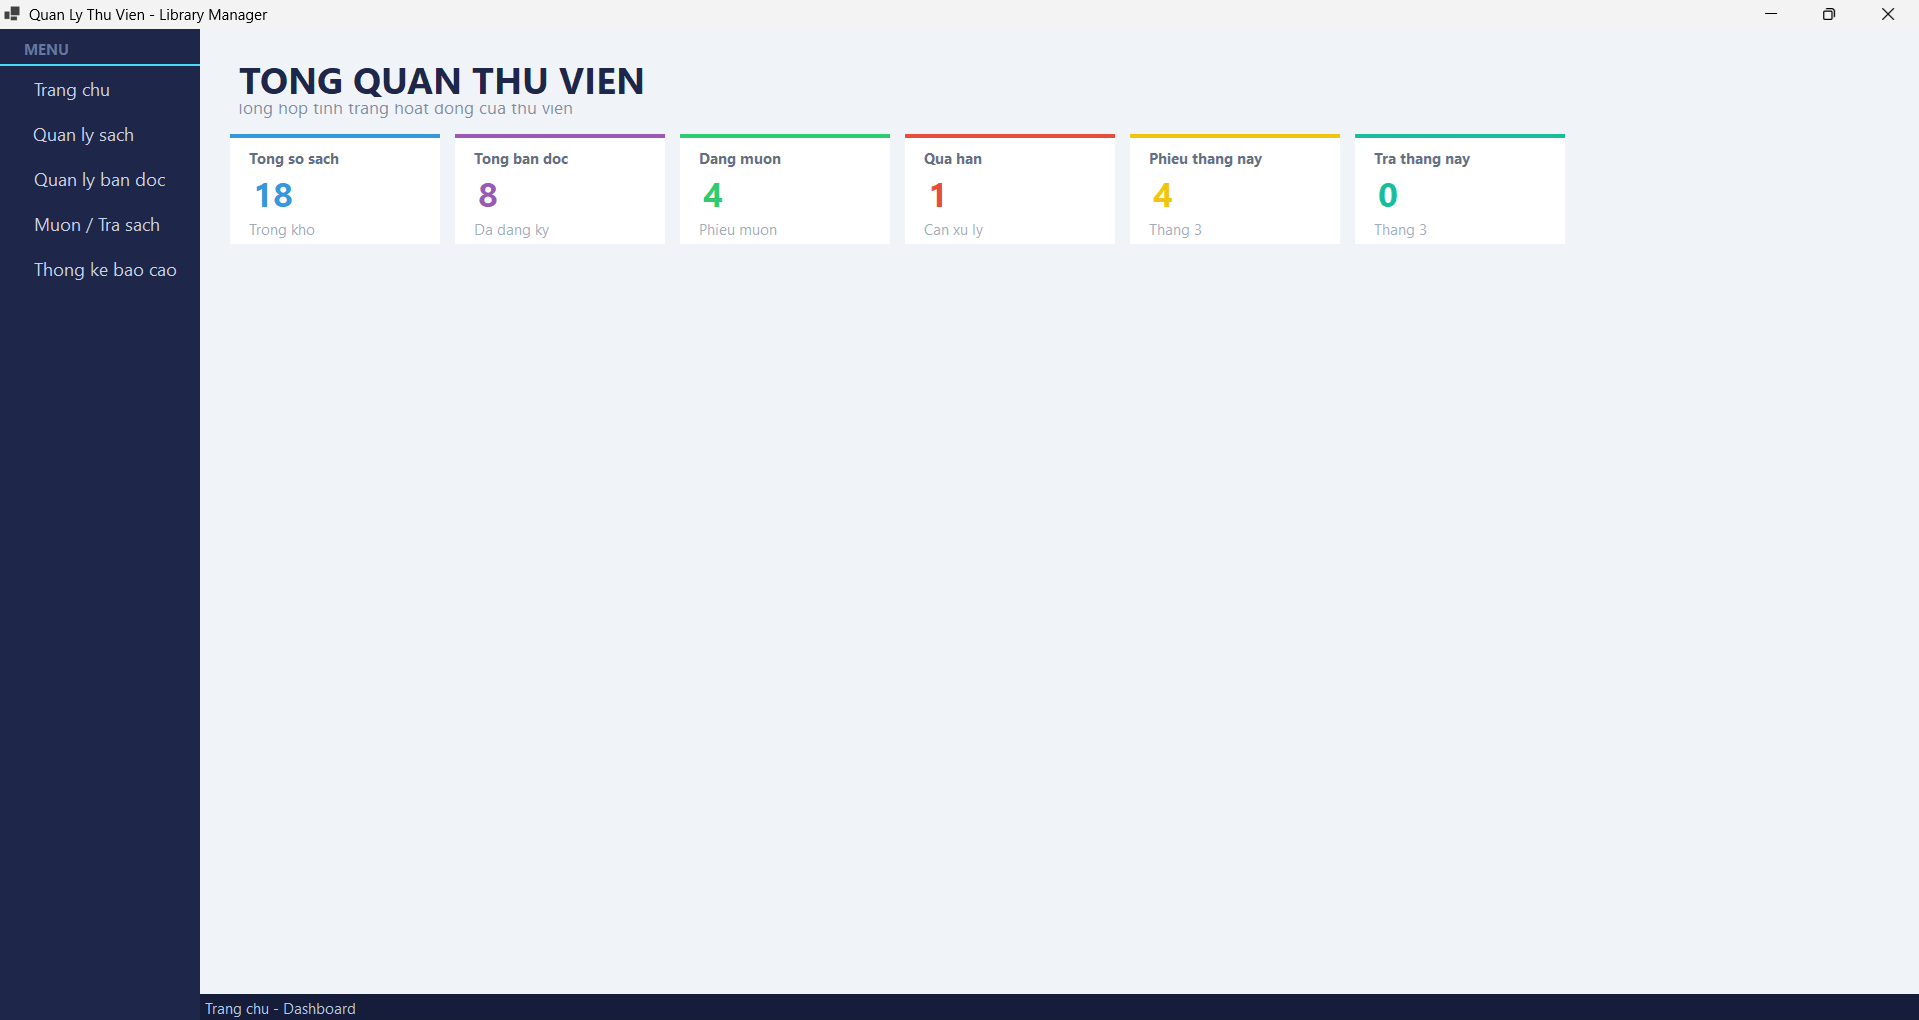
\includegraphics[width=\textwidth]{trangchu_tongquanthuvien.png}
    \caption{Main dashboard displaying real-time library operational indicators.}
    \label{fig:dashboard}
\end{figure}

\subsection{Book Management}
\subsubsection{Book Catalog View}
Figure~\ref{fig:book_list} presents the book management screen with the full catalog displayed in a sortable data grid. Each row shows the book ID, title, author, category, publisher, publication year, total copies, available copies, and active status. The search bar at the top supports combined filtering by title keyword, category dropdown, and author text field. The input form at the bottom allows direct data entry for new records or editing of selected records. This screen satisfies FR1.

\begin{figure}[H]
    \centering
    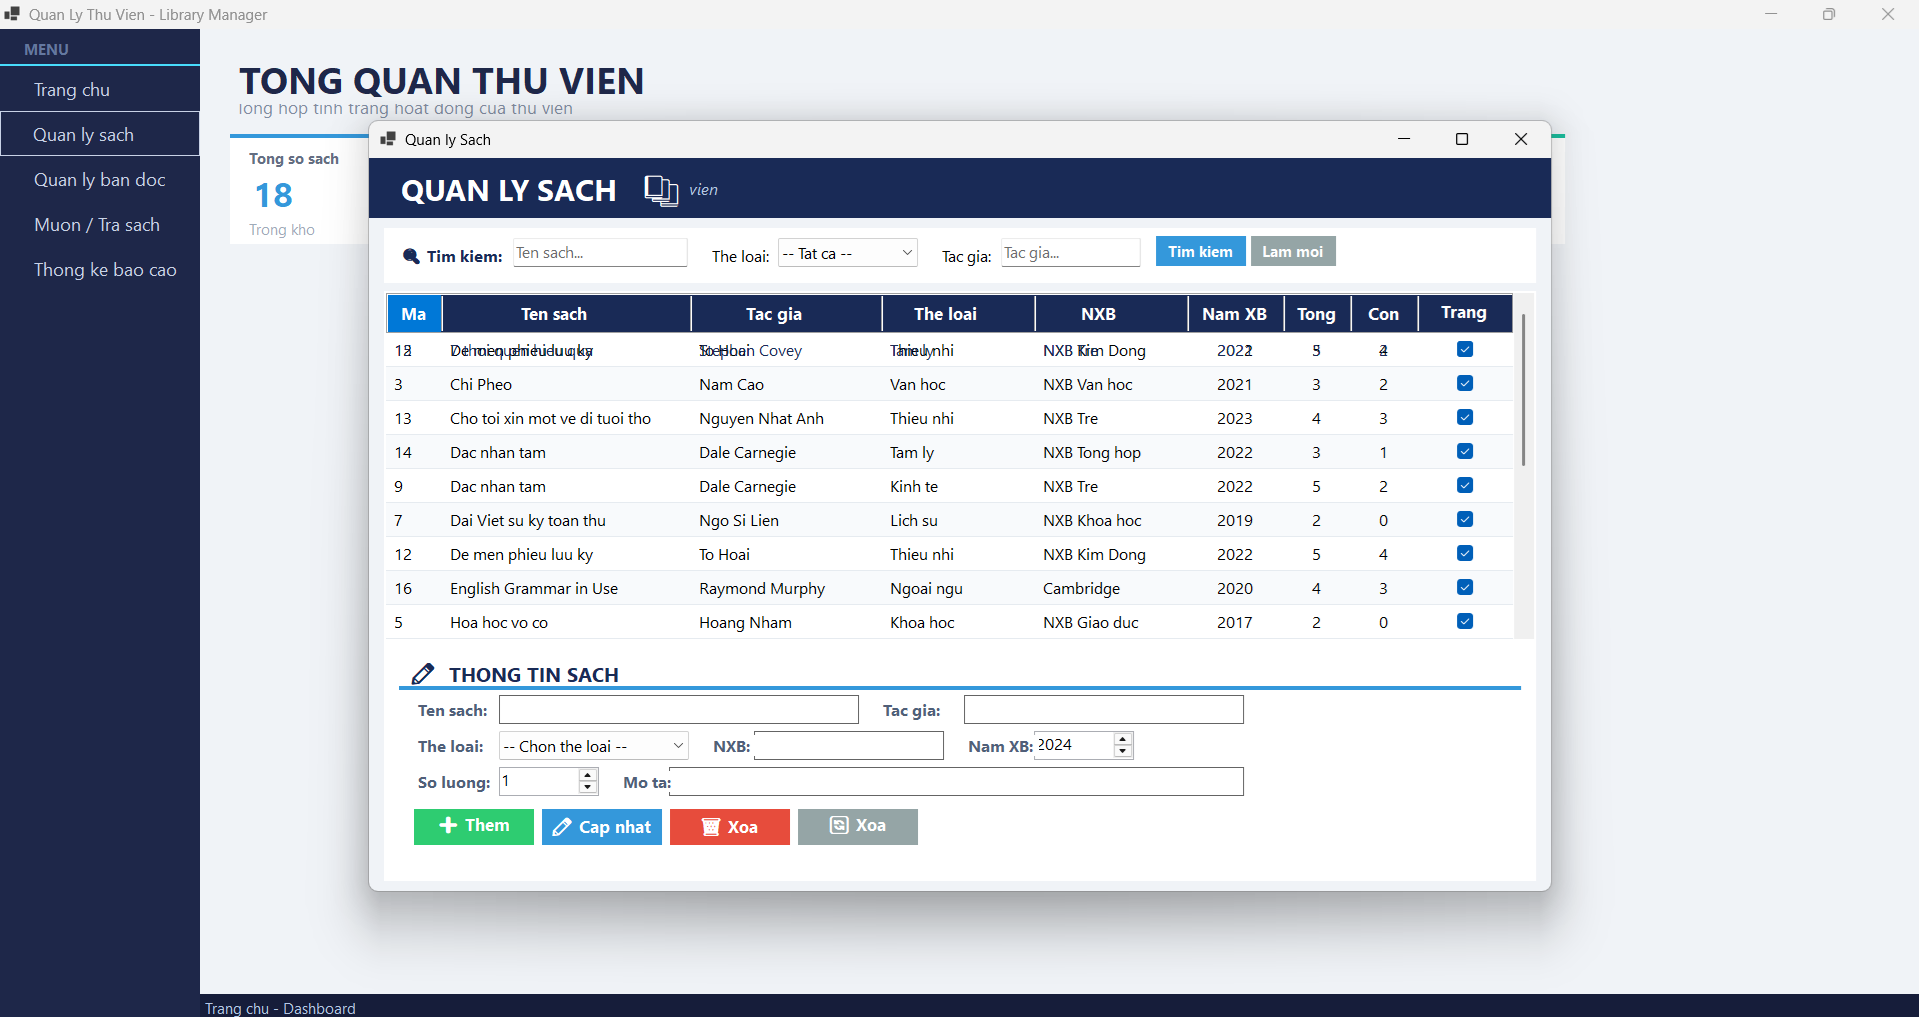
\includegraphics[width=\textwidth]{quanlysach_dashboard.png}
    \caption{Book management interface with catalog grid and input form.}
    \label{fig:book_list}
\end{figure}

\subsubsection{Adding a New Book}
Figure~\ref{fig:book_add} demonstrates the successful creation of a new book record. The operator entered the title ``Cay cam ngot cua toi'' by author ``HNMU'', assigned to the ``Van hoc'' category, published by ``NXB Nha Nam'' in 2024, with 1 copy. The system confirms success with a dialog showing the generated book ID (Ma sach: 19). The BLL validated all required fields before executing the insert operation.

\begin{figure}[H]
    \centering
    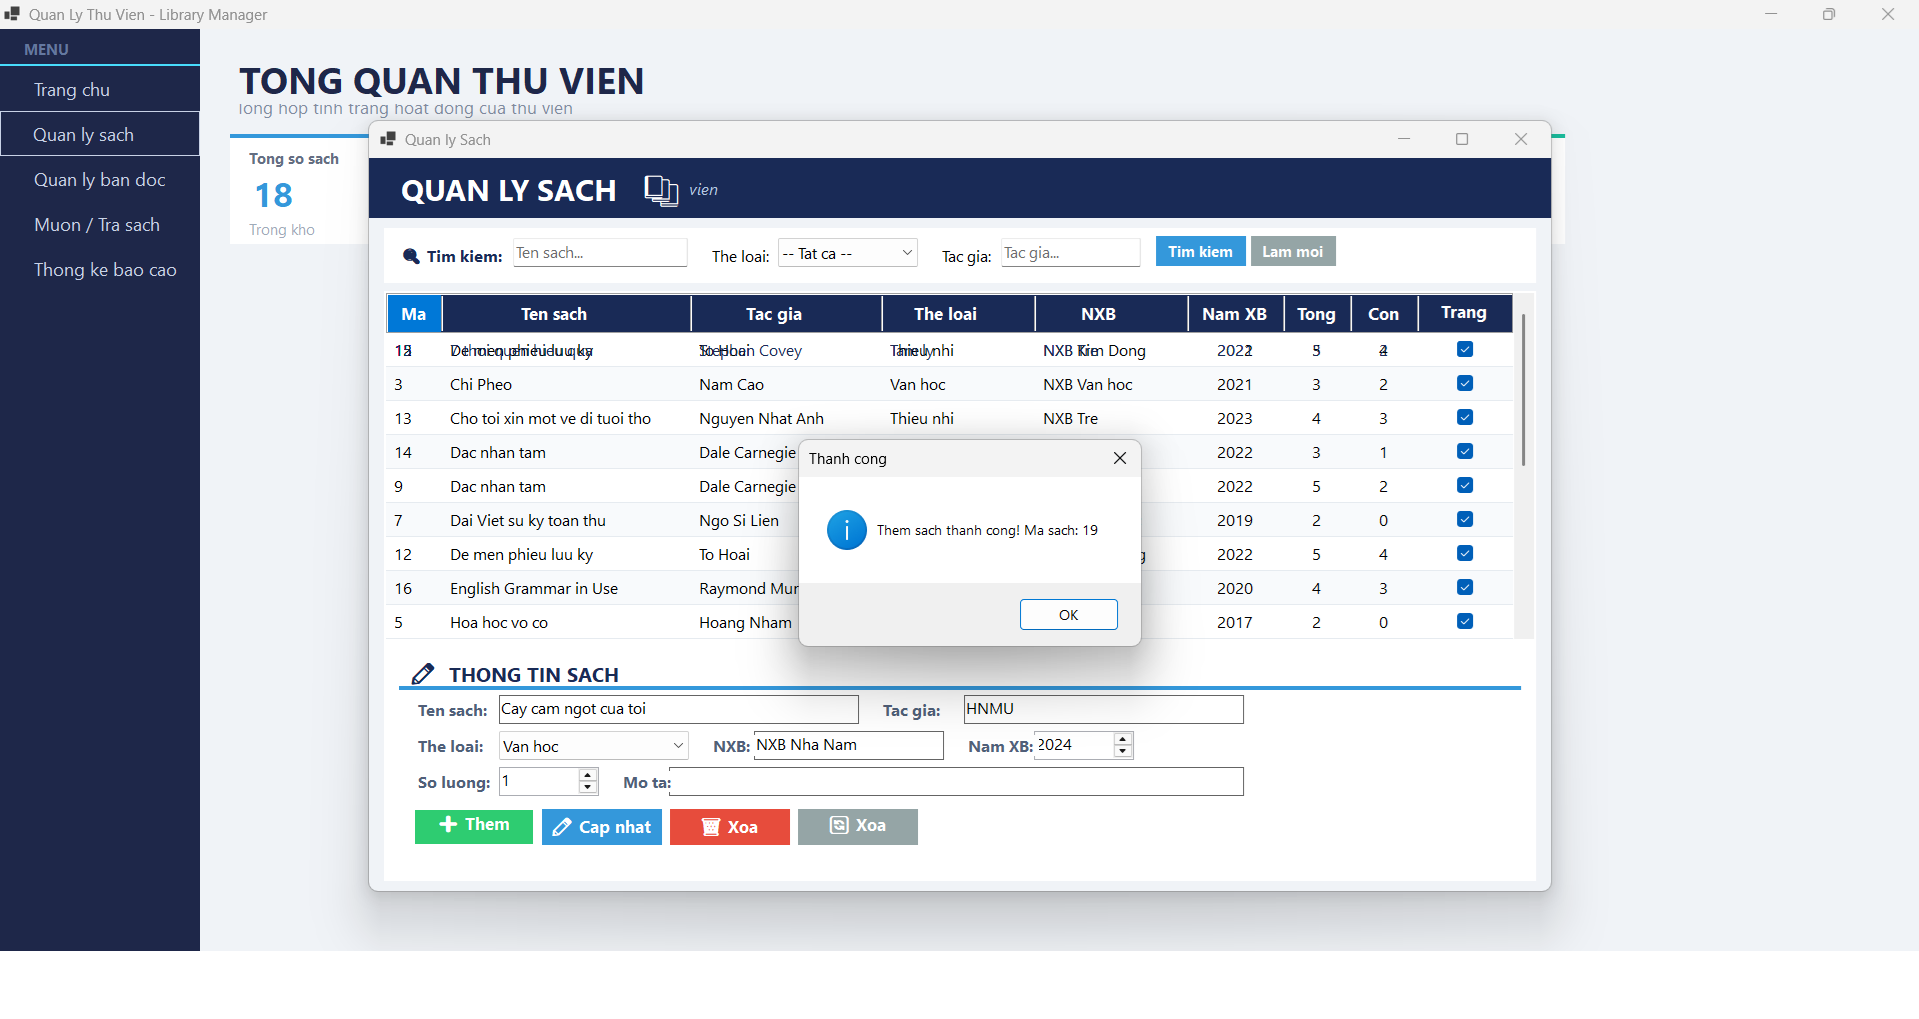
\includegraphics[width=\textwidth]{quanlysach_themsach.png}
    \caption{Successful book creation with auto-generated ID confirmation.}
    \label{fig:book_add}
\end{figure}

\subsubsection{Updating Book Information}
Figure~\ref{fig:book_update} shows the update workflow. The operator selected ``Cho toi xin mot ve di tuoi tho'' from the grid, modified the quantity to 3, and submitted the update. The success dialog confirms the operation. The BLL automatically recalculated \texttt{SoLuongCon} based on the change in total quantity, demonstrating the proportional stock adjustment logic described in Section 5.3.

\begin{figure}[H]
    \centering
    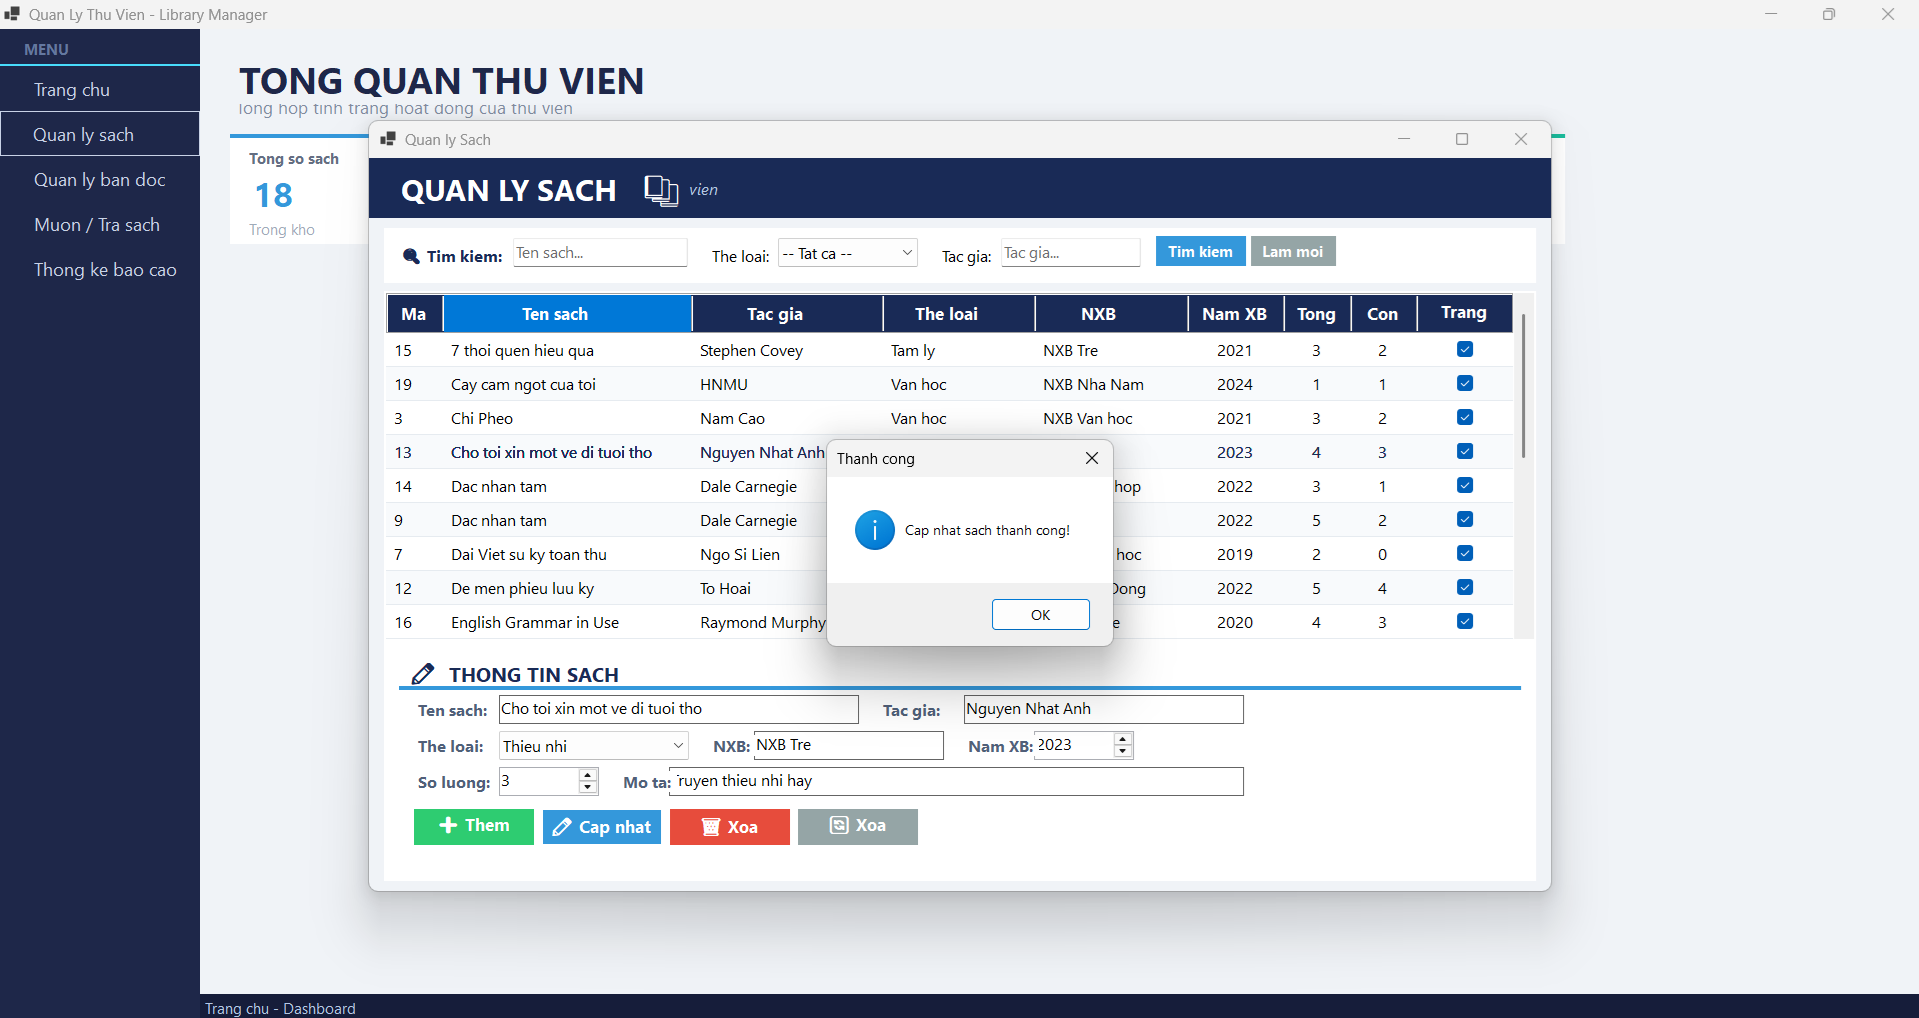
\includegraphics[width=\textwidth]{quanlysach_capnhatsach.png}
    \caption{Book update operation with automatic stock recalculation.}
    \label{fig:book_update}
\end{figure}

\subsubsection{Deleting a Book}
Figure~\ref{fig:book_delete} illustrates the deletion confirmation dialog. The operator selected ``Dac nhan tam'' and initiated deletion. The system prompts a Yes/No confirmation to prevent accidental data loss. If the book has existing borrowing references, the operation would be blocked with an appropriate error message due to foreign-key constraints.

\begin{figure}[H]
    \centering
    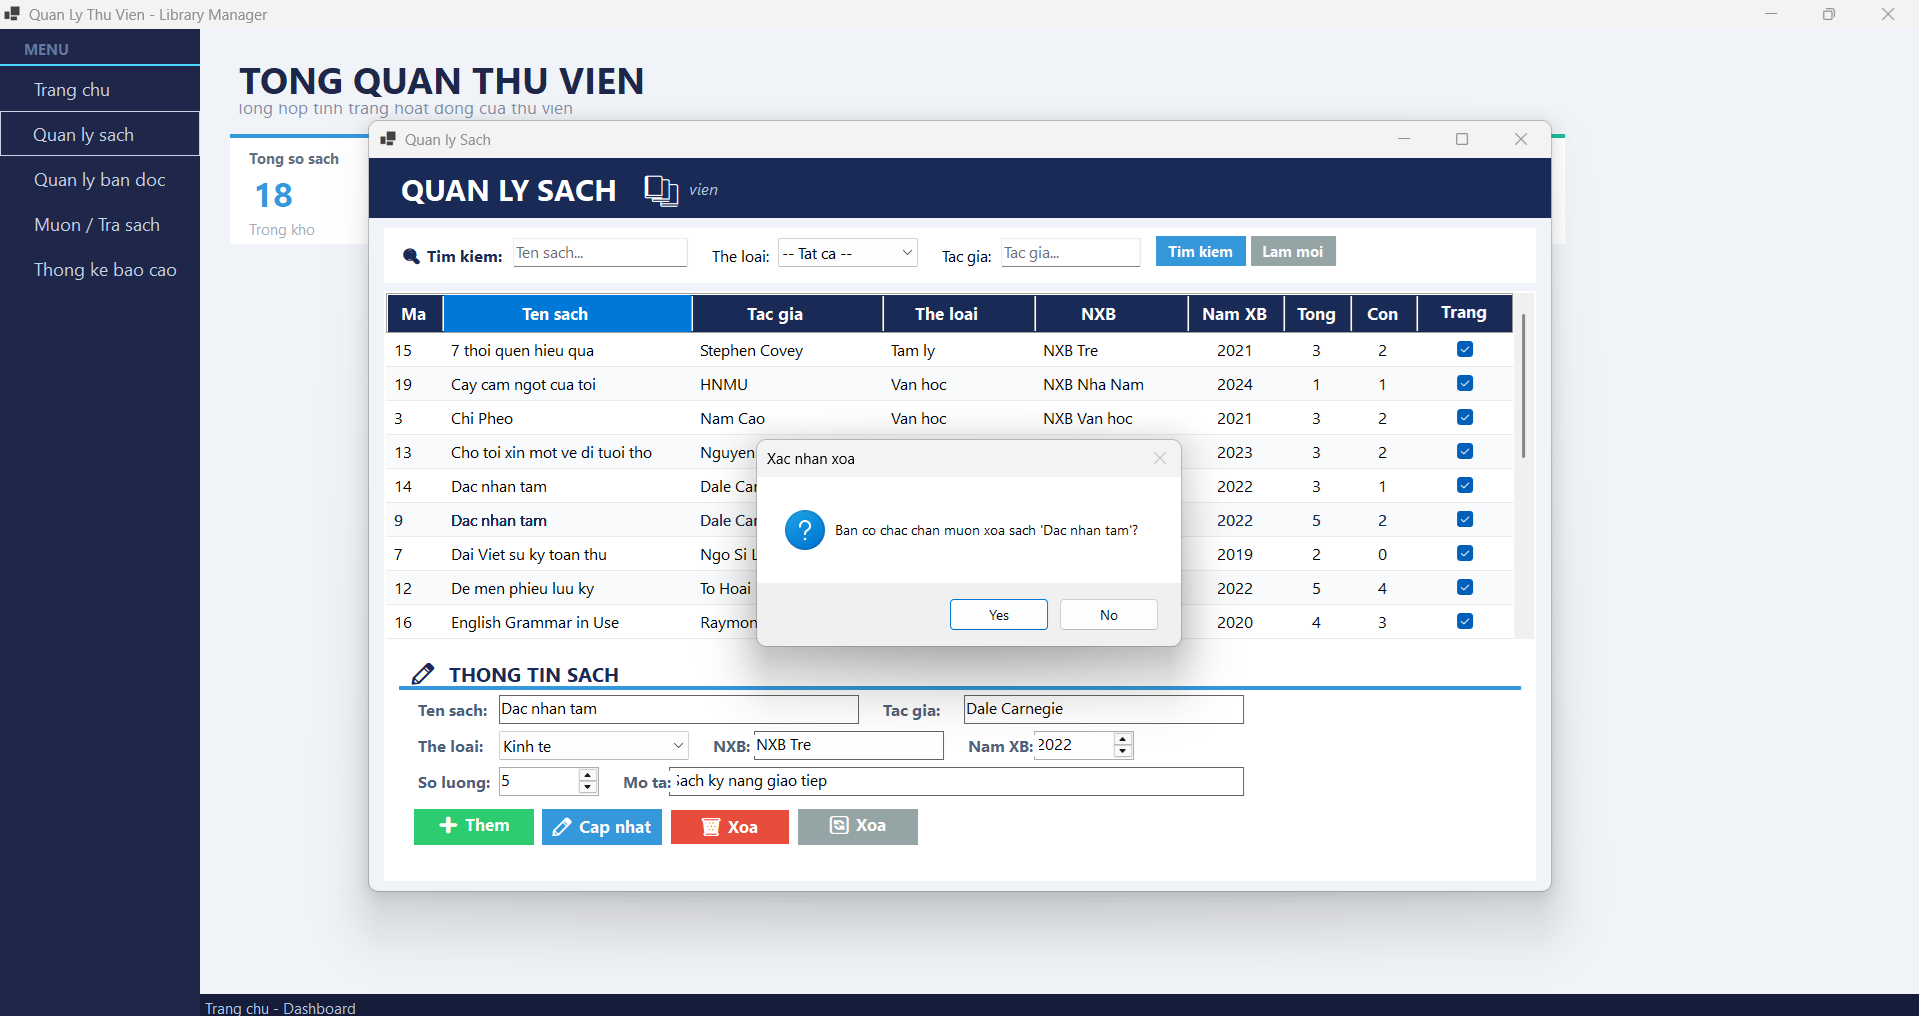
\includegraphics[width=\textwidth]{quanlysach_xoasach.png}
    \caption{Book deletion with confirmation dialog and referential integrity check.}
    \label{fig:book_delete}
\end{figure}

\subsection{Reader Management}
\subsubsection{Reader List View}
Figure~\ref{fig:reader_list} shows the reader management interface with the complete list of registered readers. The grid displays reader ID, full name, date of birth, gender, phone number, email, address, registration date, and status. The input form below supports direct entry for new readers or modification of selected records. This screen satisfies FR2.

\begin{figure}[H]
    \centering
    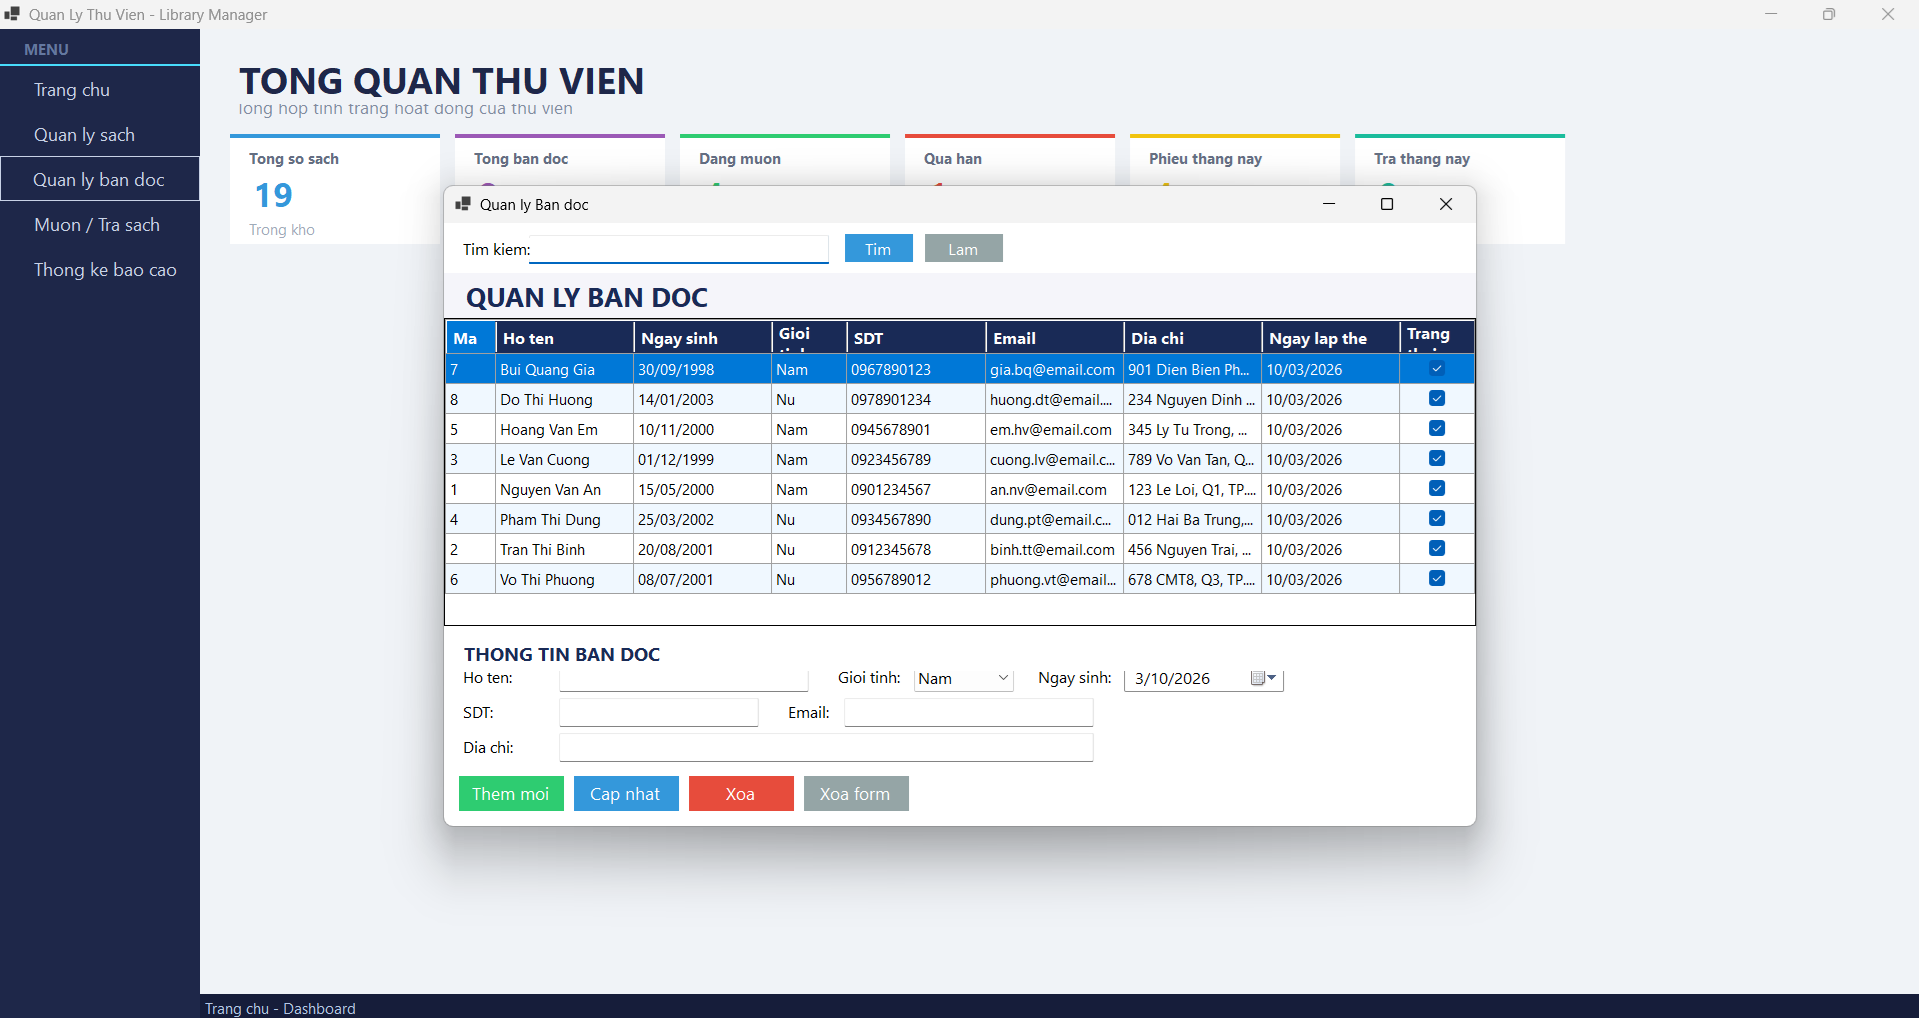
\includegraphics[width=\textwidth]{quanlybandoc_dashboard.png}
    \caption{Reader management interface with profile grid and input panel.}
    \label{fig:reader_list}
\end{figure}

\subsubsection{Adding a New Reader}
Figure~\ref{fig:reader_add} shows the successful registration of a new reader ``Hoang Kim Long'' with phone, email, and address details. The system assigned reader ID 9 and confirmed with a success dialog. The BLL verified that the full name field was non-empty before proceeding with the insert.

\begin{figure}[H]
    \centering
    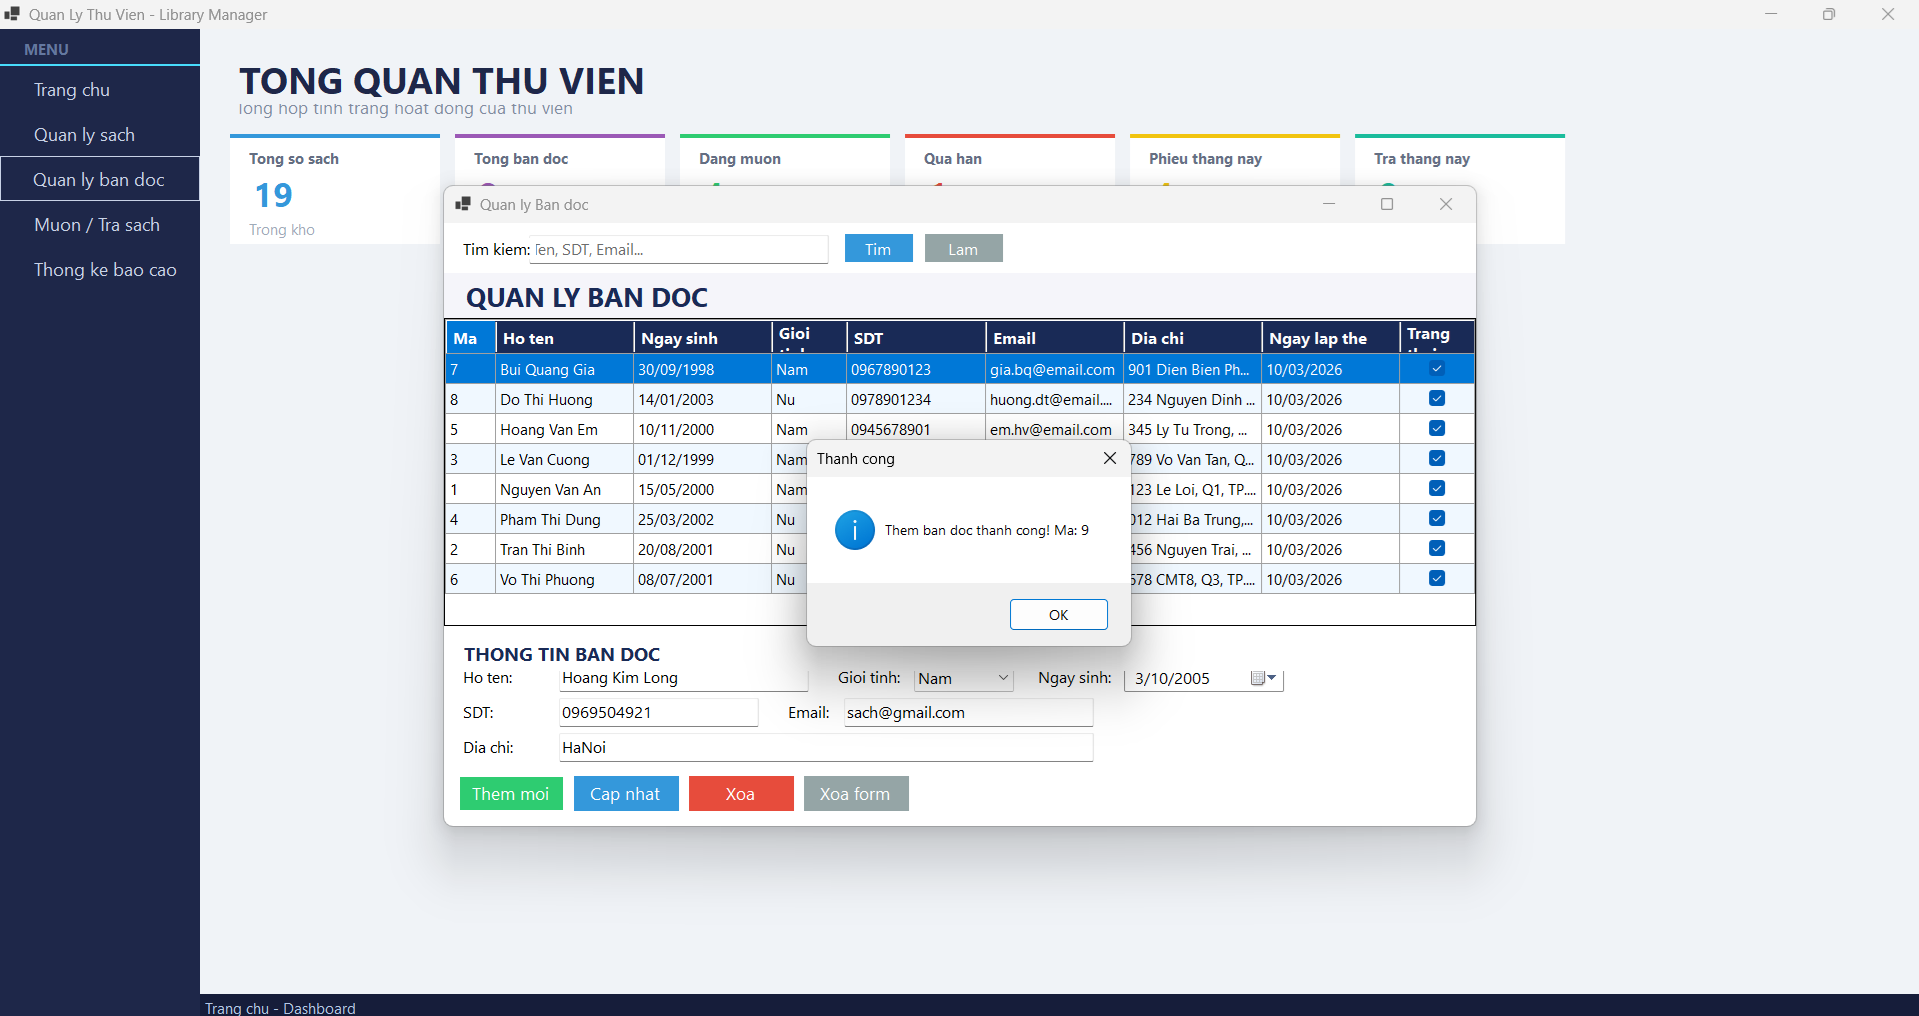
\includegraphics[width=\textwidth]{quanlybandoc_them.png}
    \caption{Successful reader registration with generated ID confirmation.}
    \label{fig:reader_add}
\end{figure}

\subsubsection{Updating Reader Information}
Figure~\ref{fig:reader_update} demonstrates updating an existing reader record (``Pham Thi Dung''). The operator modified profile fields and received a success confirmation. The grid immediately refreshes to display the updated data.

\begin{figure}[H]
    \centering
    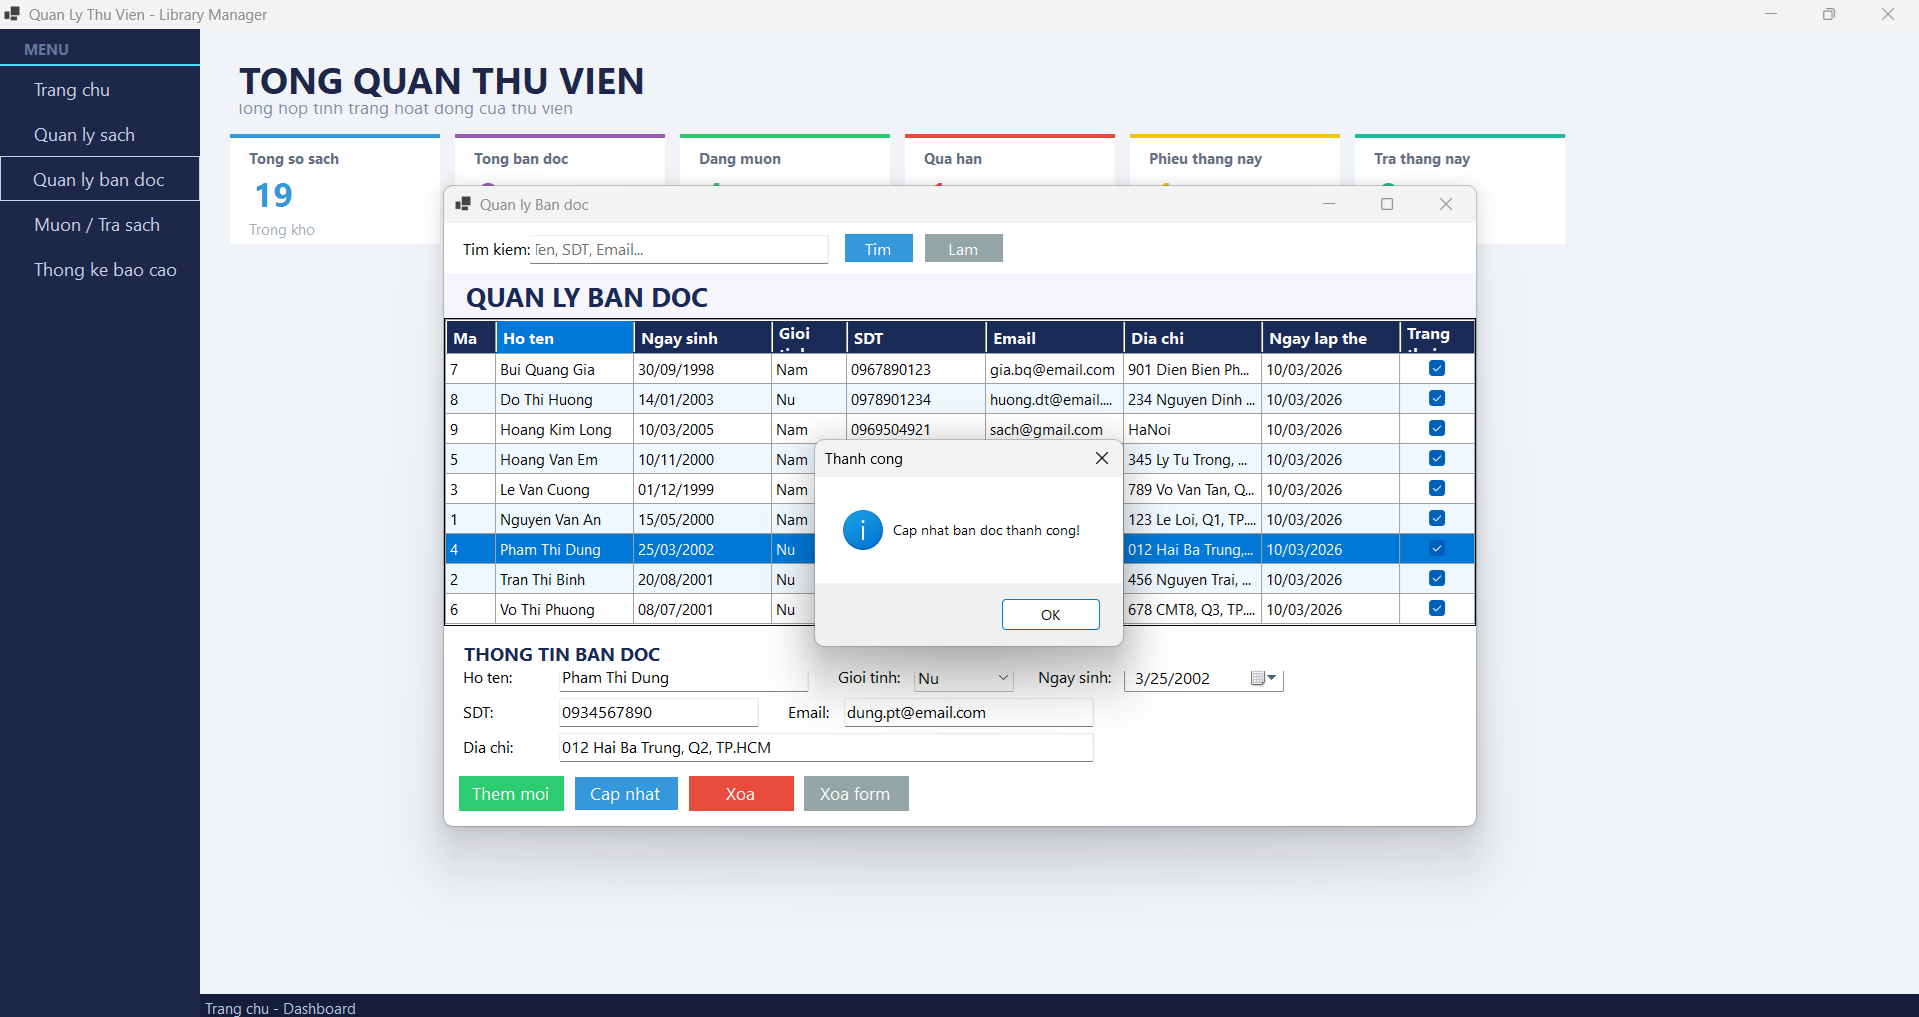
\includegraphics[width=\textwidth]{quanlybandoc_capnhat.png}
    \caption{Reader profile update with success confirmation.}
    \label{fig:reader_update}
\end{figure}

\subsubsection{Deleting a Reader}
Figure~\ref{fig:reader_delete} shows the deletion confirmation dialog for reader ``Vo Thi Phuong''. The system requires explicit Yes/No confirmation. If the reader currently has active borrowed books, the BLL would reject the operation with a descriptive error message, enforcing the dependency constraint.

\begin{figure}[H]
    \centering
    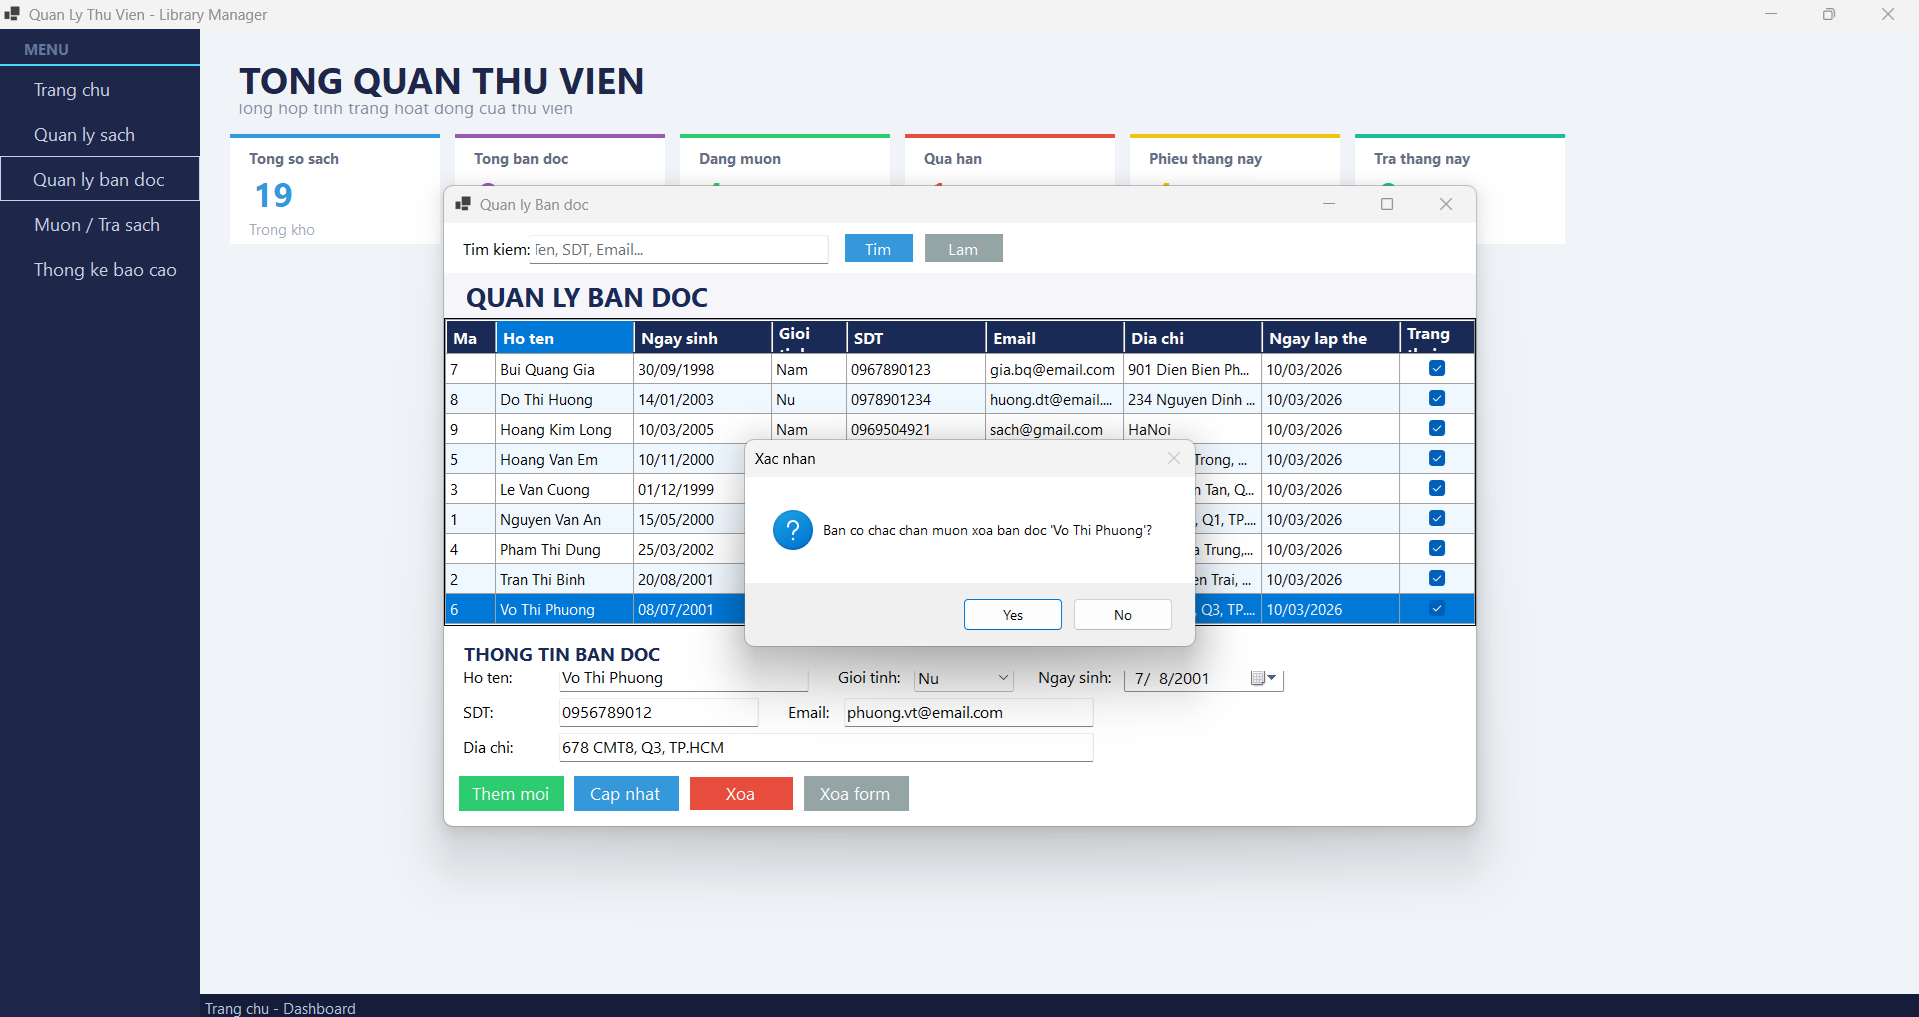
\includegraphics[width=\textwidth]{quanlybandoc_xoa.png}
    \caption{Reader deletion with confirmation prompt and dependency check.}
    \label{fig:reader_delete}
\end{figure}

\subsection{Borrow/Return Workflow}
\subsubsection{Borrowing Ticket List}
Figure~\ref{fig:borrow_list} presents the circulation management screen. The left panel displays all borrowing tickets with color-coded status: blue for active (``Dang muon''), red-highlighted for overdue (``Qua han''), and default for returned (``Da tra''). The right panel provides two tabs: ``Lap phieu muon'' for creating new tickets and ``Chi tiet phieu'' for viewing details of a selected ticket. The search bar supports filtering by ticket ID, reader name, and status. This screen satisfies FR3, FR4, and FR5.

\begin{figure}[H]
    \centering
    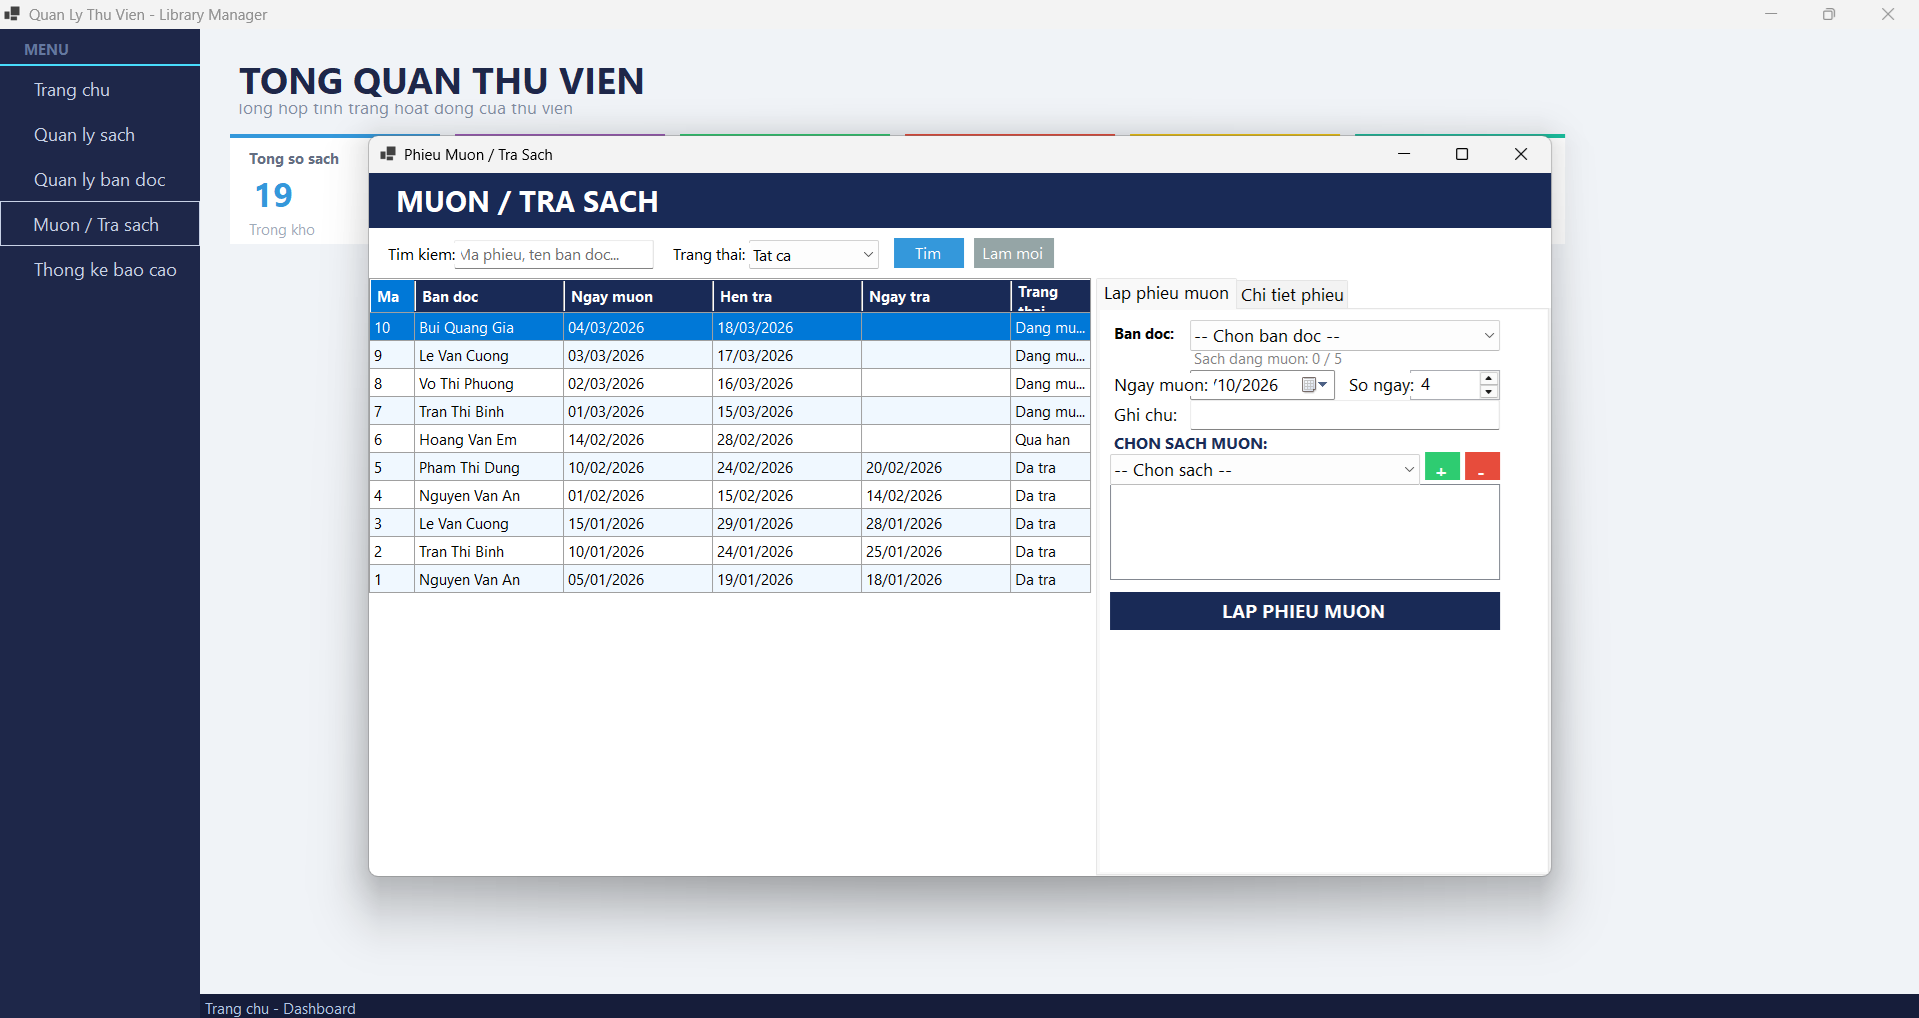
\includegraphics[width=\textwidth]{muontrasach_dashboard.png}
    \caption{Circulation management interface with ticket list and tabbed operations panel.}
    \label{fig:borrow_list}
\end{figure}

\subsubsection{Creating a New Borrowing Ticket}
Figure~\ref{fig:borrow_create} demonstrates creating a new borrowing ticket for reader ``Hoang Kim Long''. The operator selected one book (``TOEIC 990'') and submitted the ticket. The system validated the reader's current borrowing count (displayed as ``Sach dang muon: 0 / 5''), verified book availability, and confirmed successful creation with ticket ID 11. The book's \texttt{SoLuongCon} was automatically decremented.

\begin{figure}[H]
    \centering
    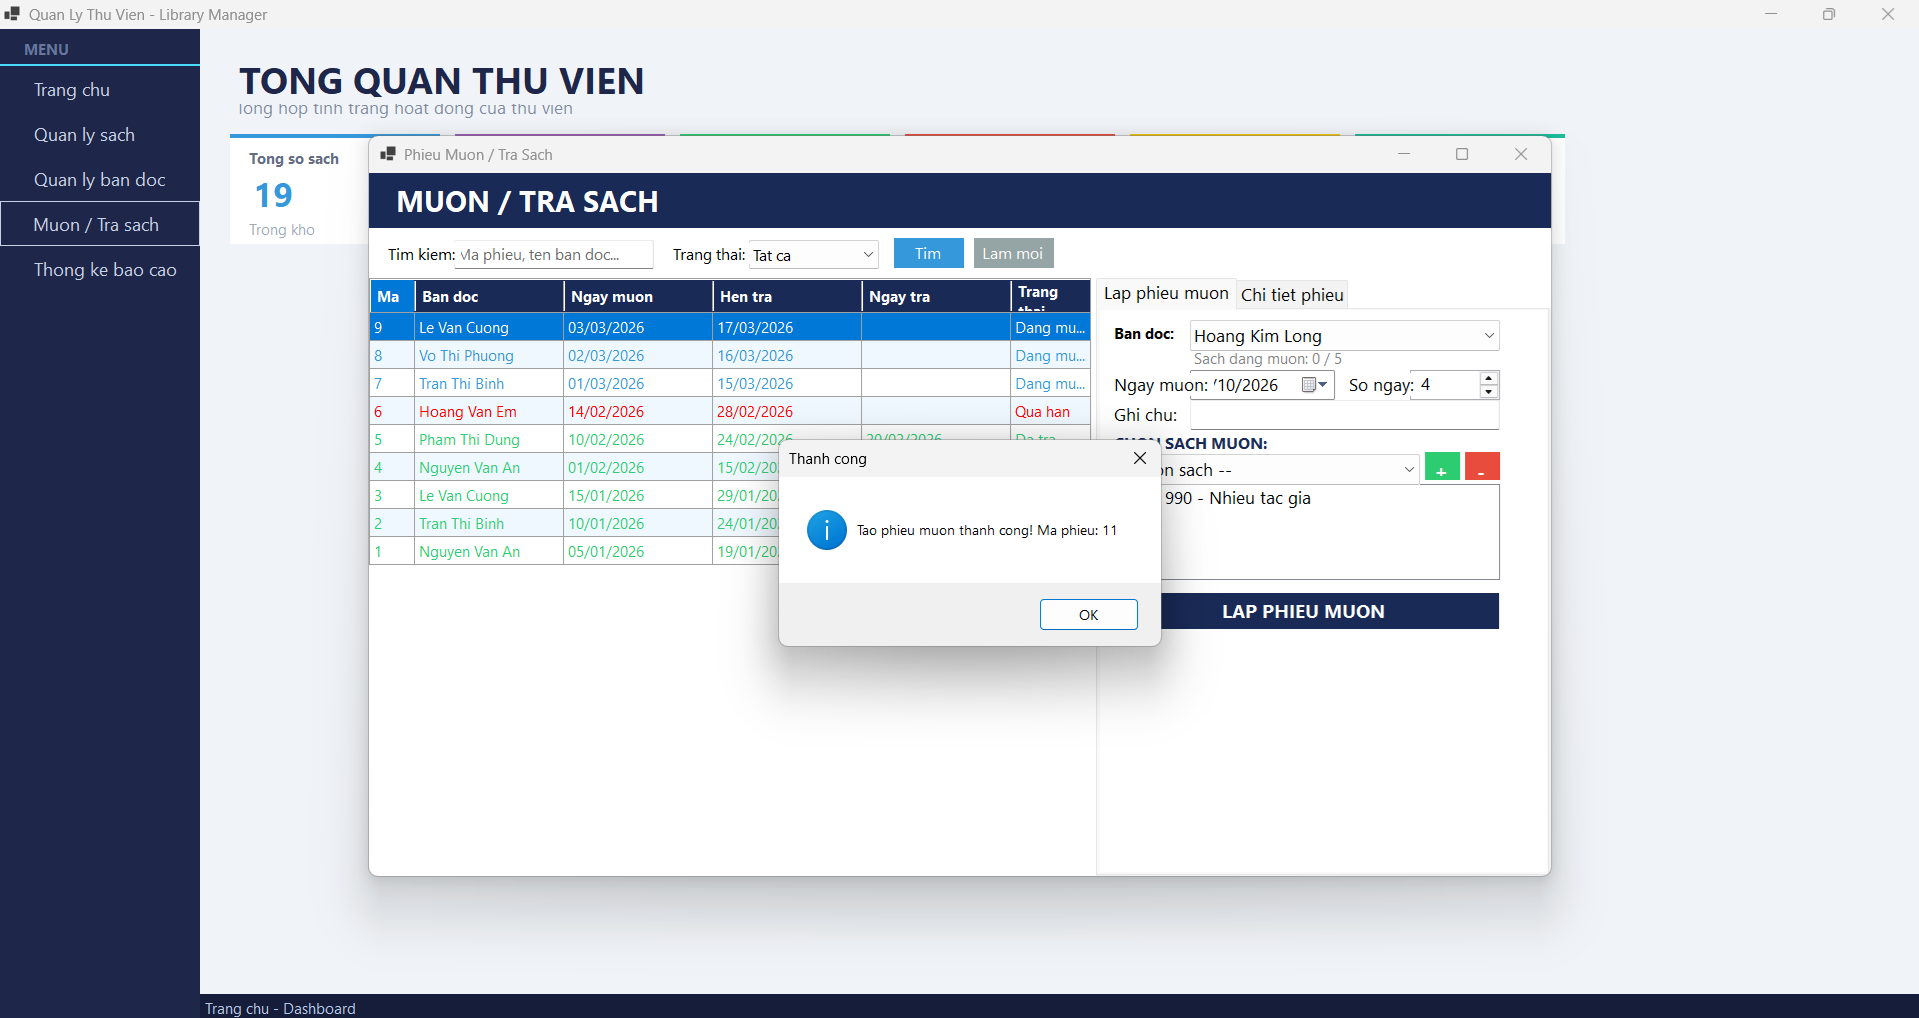
\includegraphics[width=\textwidth]{muontrasach_lapphieumuon.png}
    \caption{Borrowing ticket creation with reader validation and success confirmation.}
    \label{fig:borrow_create}
\end{figure}

\subsubsection{Returning Books}
Figure~\ref{fig:return_confirm} shows the return confirmation dialog. The operator selected ticket \#10 belonging to ``Bui Quang Gia'' and clicked ``TRA SACH''. The right panel displays the ticket details: two books (``Nhat ky trong tu'' and ``Dac nhan tam'') with their current return status. The system prompts a Yes/No confirmation before executing the transactional return.

\begin{figure}[H]
    \centering
    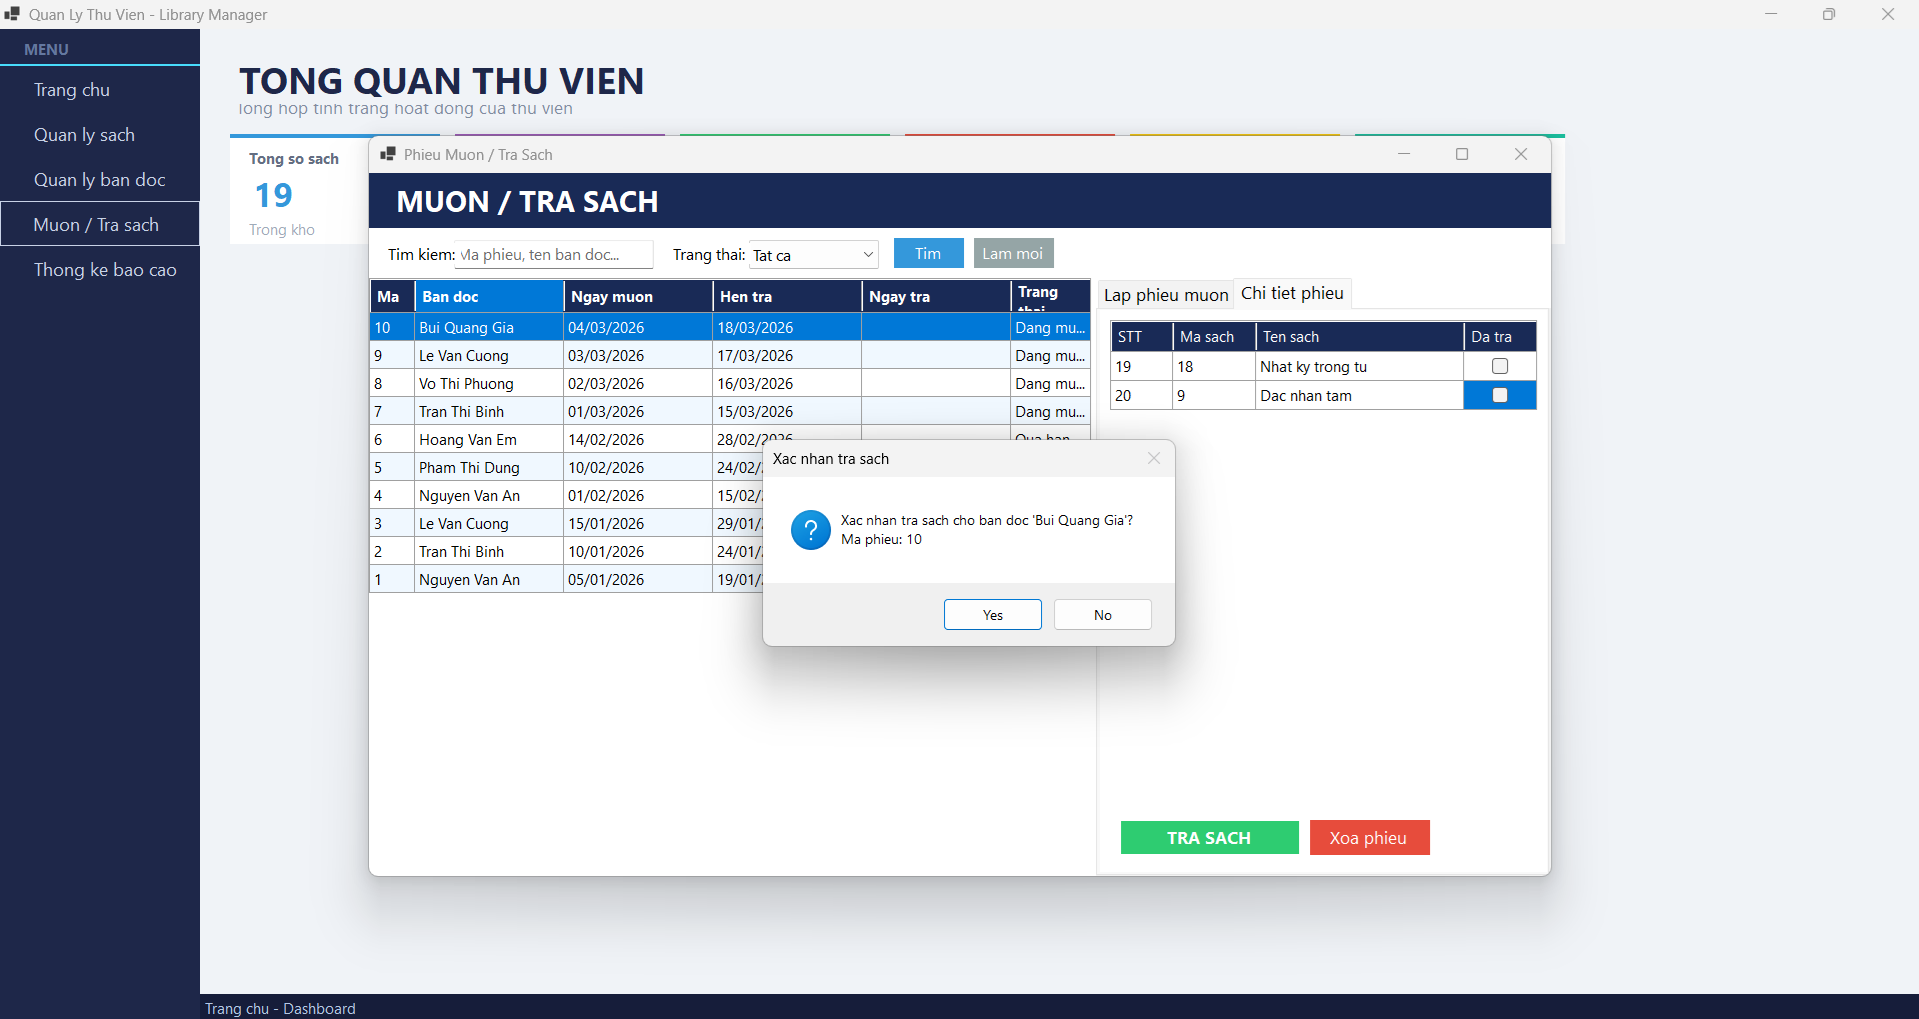
\includegraphics[width=\textwidth]{muontrasach_trasach.png}
    \caption{Return confirmation dialog with ticket detail inspection.}
    \label{fig:return_confirm}
\end{figure}

Figure~\ref{fig:return_success} shows the success notification after the return transaction completed. The ticket status has been updated to ``Da tra'', the actual return date is recorded, and inventory counts for both books have been restored. This demonstrates the atomic transaction behavior described in Section 5.6.

\begin{figure}[H]
    \centering
    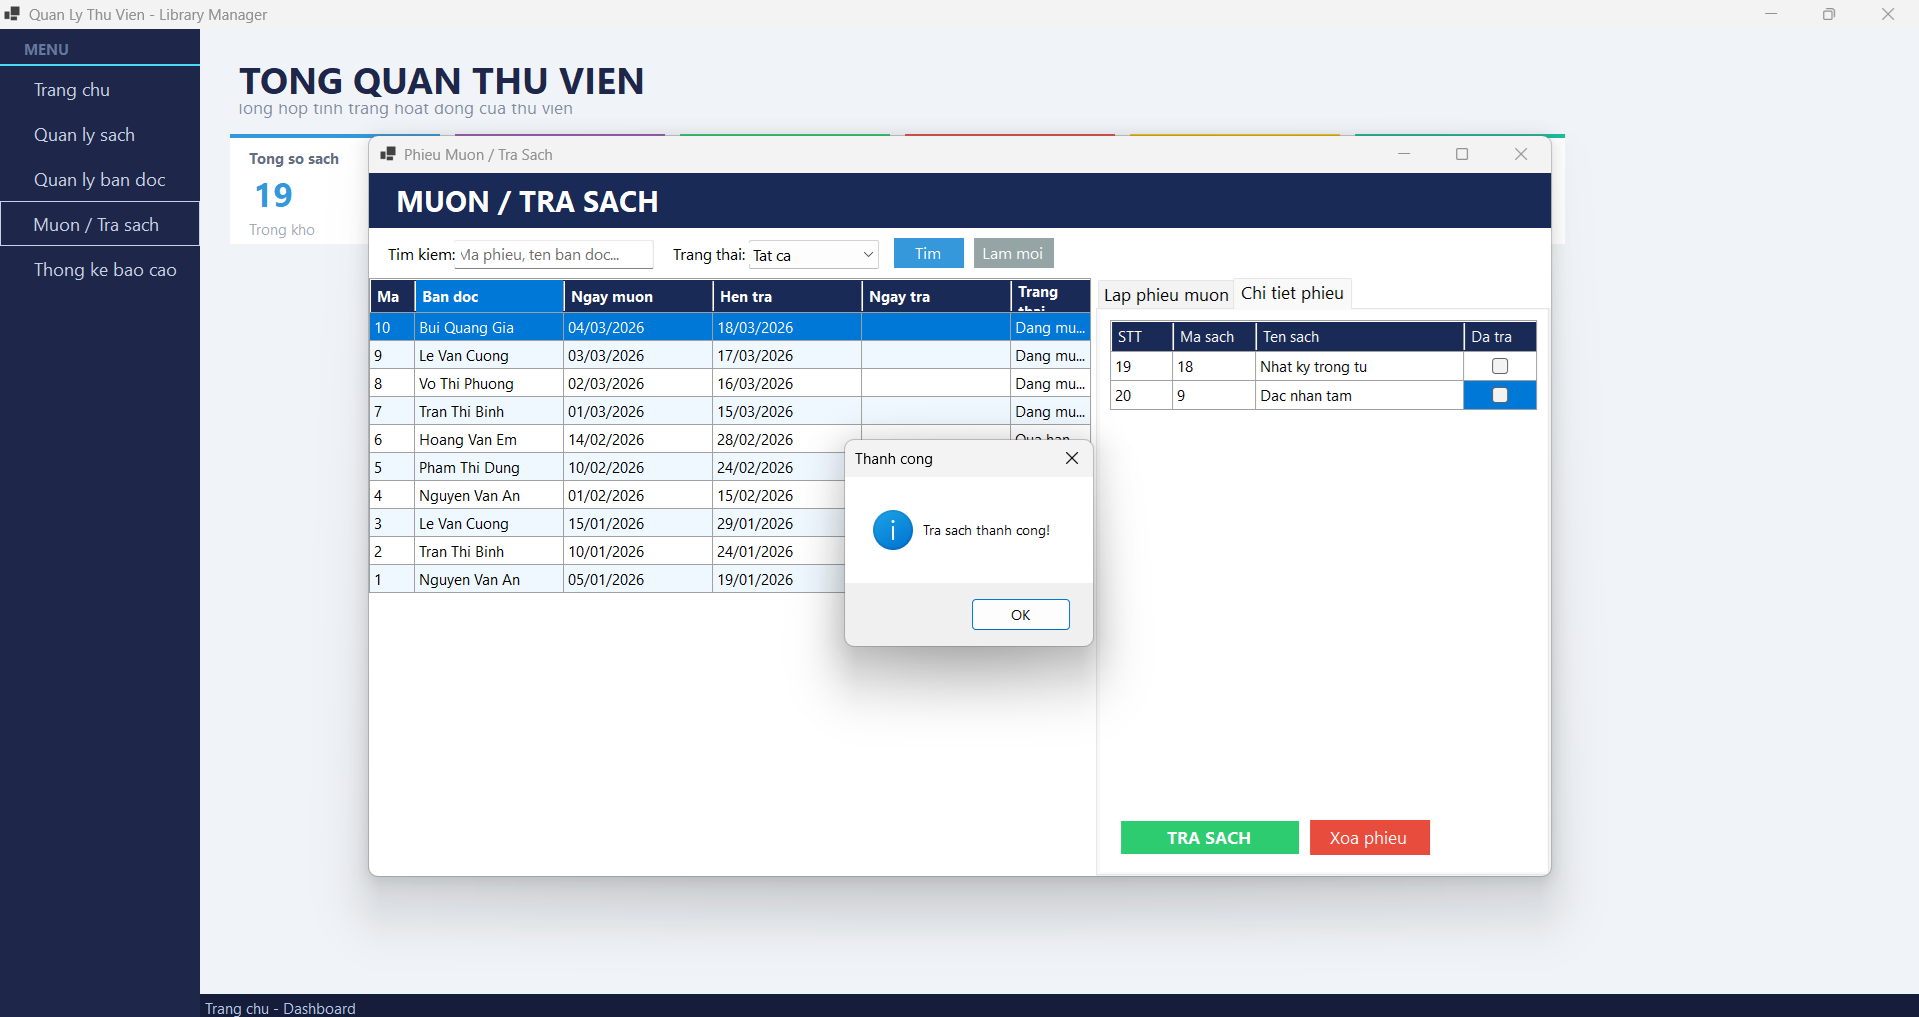
\includegraphics[width=\textwidth]{muontrasach_trasach_thanhcong.png}
    \caption{Successful return with transaction-safe status and inventory update.}
    \label{fig:return_success}
\end{figure}

\subsubsection{Deleting a Completed Ticket}
Figure~\ref{fig:ticket_delete} shows the ticket deletion workflow. After ticket \#10 was returned, the operator can optionally delete the completed ticket. The system prompts for confirmation. Deletion of tickets that are still active (``Dang muon'' or ``Qua han'') would be rejected by the BLL.

\begin{figure}[H]
    \centering
    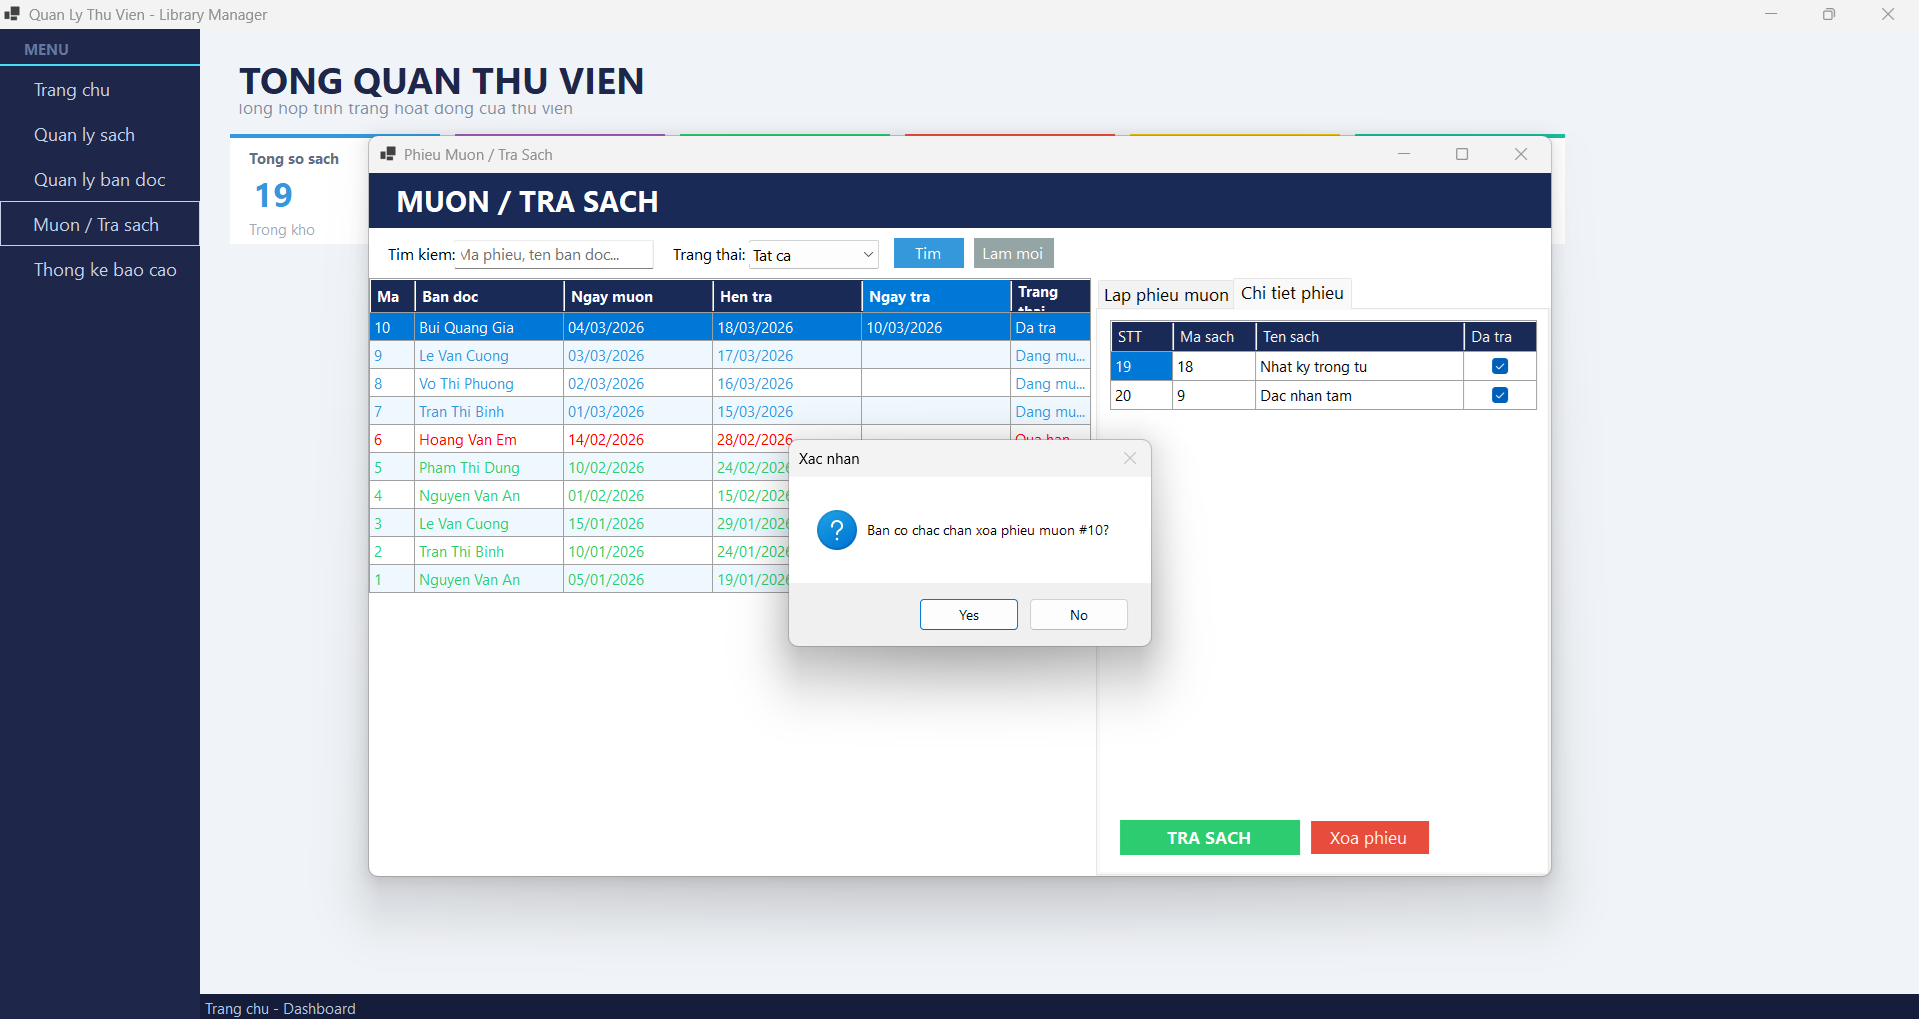
\includegraphics[width=\textwidth]{muontrasach_xoaphieu.png}
    \caption{Completed ticket deletion with confirmation and status validation.}
    \label{fig:ticket_delete}
\end{figure}

\subsection{Statistics and Reporting}
\subsubsection{Statistical Dashboard}
Figure~\ref{fig:stats_dashboard} presents the statistics screen for March 2026. The summary cards show 4 total tickets, 0 returned, 4 active, 0 overdue, and 6 total borrowed books for the selected period. The monthly breakdown table displays circulation trends across January through March. The ``SACH MUON NHIEU NHAT'' section ranks the most frequently borrowed titles, with ``TOEIC 990'' leading at 2 occurrences. This satisfies FR6.

\begin{figure}[H]
    \centering
    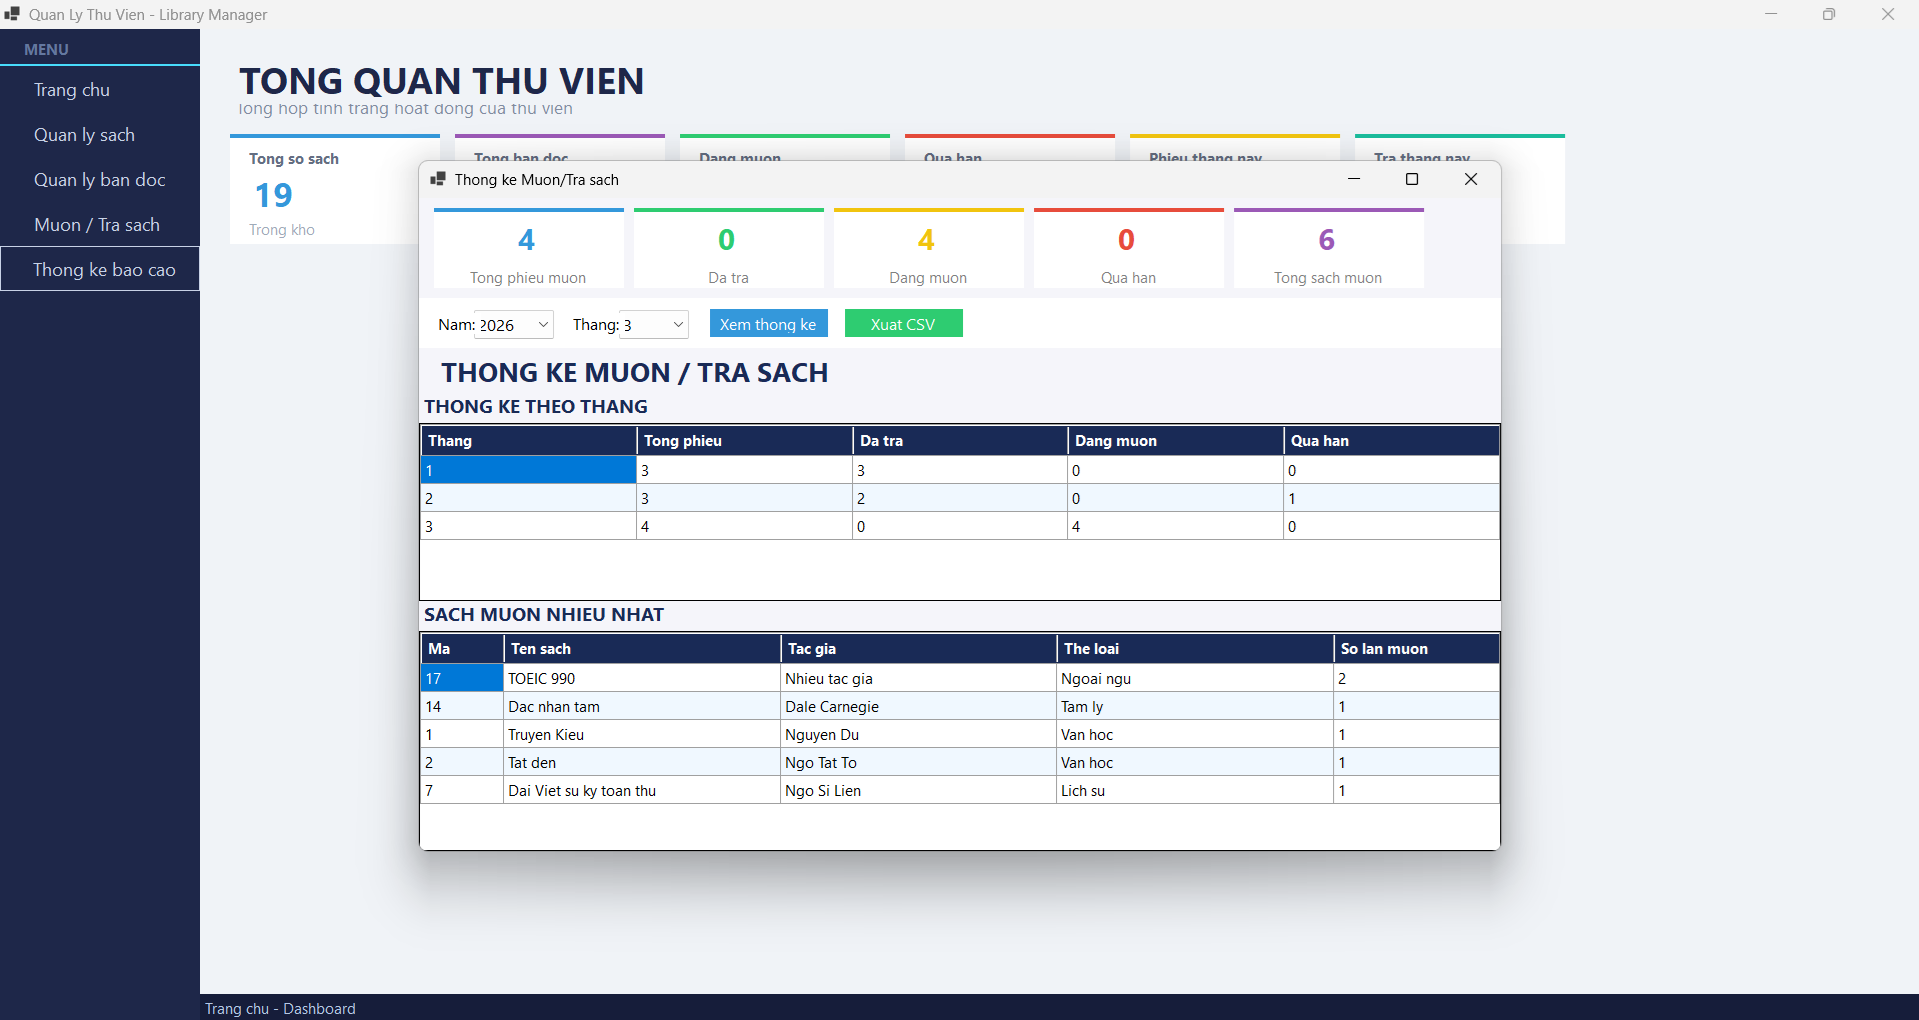
\includegraphics[width=\textwidth]{thongkebaocao_dashboard.png}
    \caption{Statistical dashboard with monthly summary, trend table, and top-book ranking.}
    \label{fig:stats_dashboard}
\end{figure}

\subsubsection{CSV Report Export}
Figure~\ref{fig:csv_export} shows the Save As dialog for exporting the monthly report as a CSV file. The default filename follows the pattern \texttt{BaoCao\_MuonTra\_\{month\}\_\{year\}.csv}. The exported file uses UTF-8 encoding with BOM to ensure correct character rendering in Microsoft Excel and other spreadsheet applications. This satisfies FR7.

\begin{figure}[H]
    \centering
    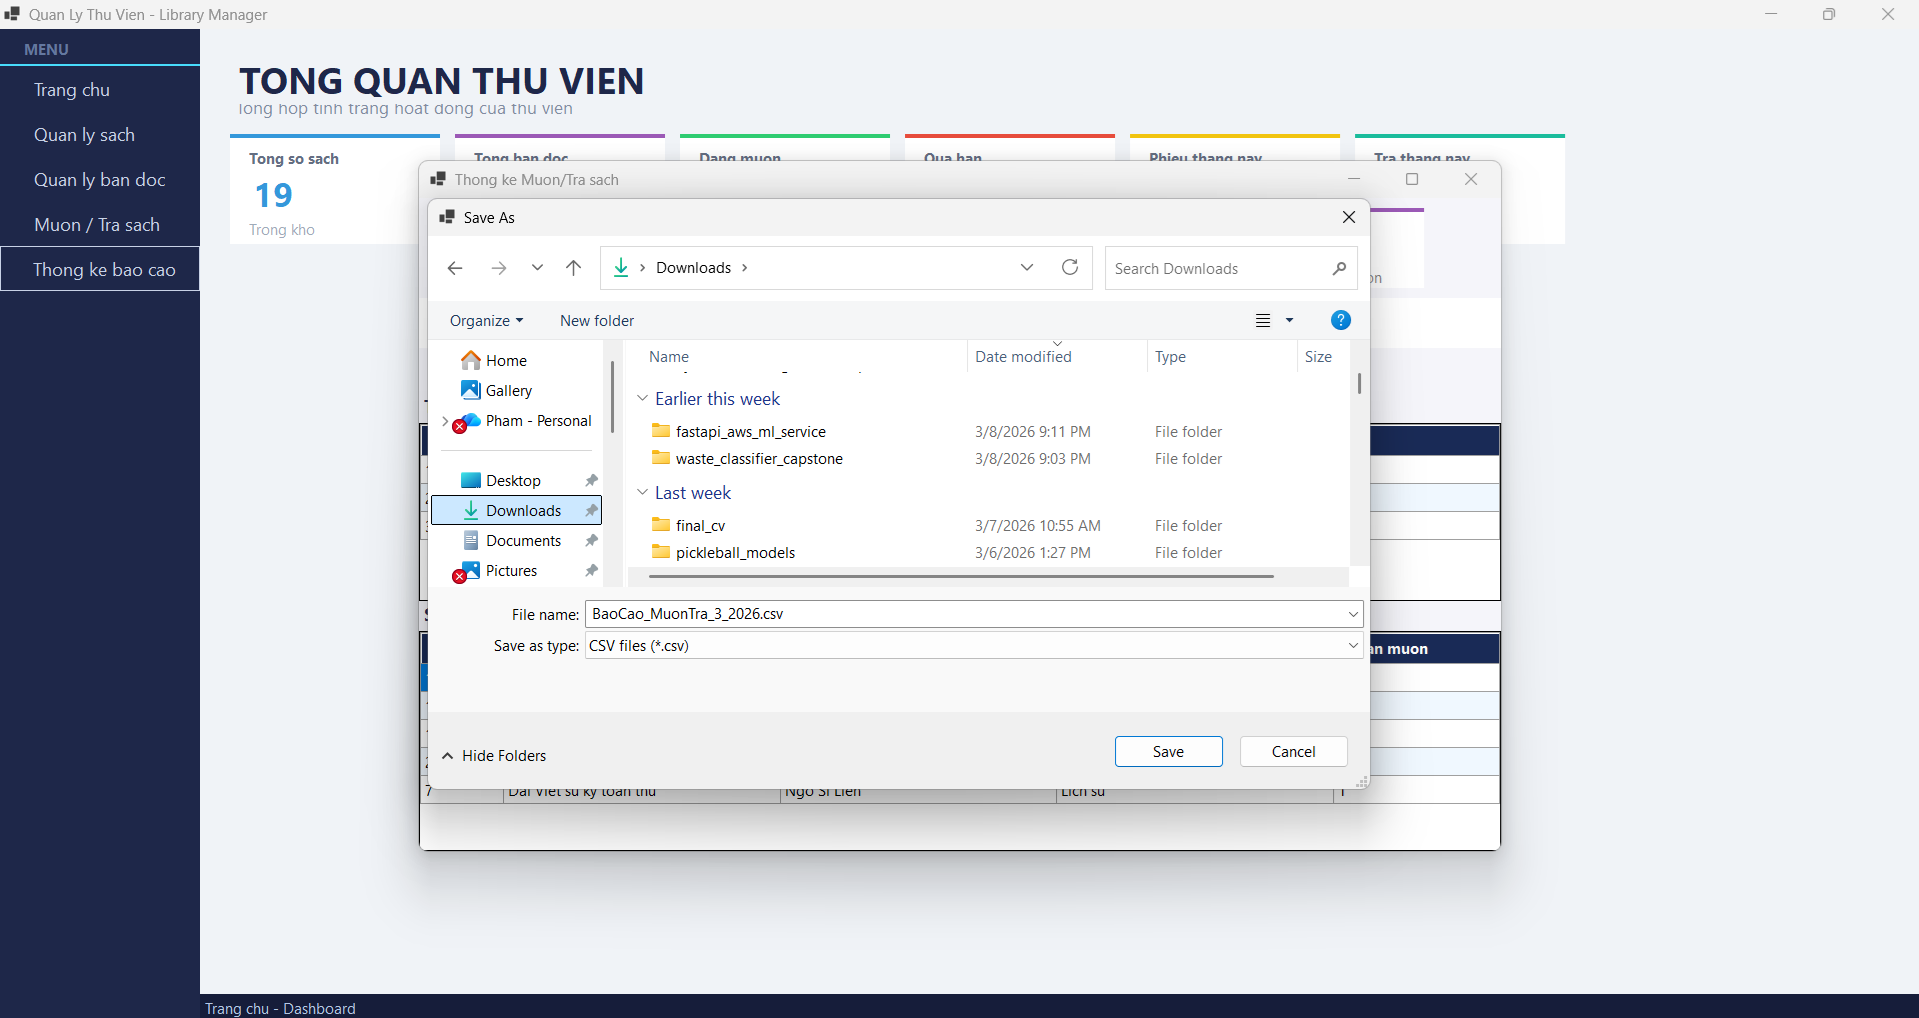
\includegraphics[width=\textwidth]{thongkebaocao_xuatcsv.png}
    \caption{CSV report export dialog with auto-generated filename.}
    \label{fig:csv_export}
\end{figure}

\subsection{Summary of Demonstrated Capabilities}
Table~\ref{tab:fr_coverage} maps each demonstrated screenshot to its corresponding functional requirement, confirming complete coverage across the product feature set.

\begin{table}[H]
\centering
\caption{Functional requirement coverage by demonstrated screenshots.}
\label{tab:fr_coverage}
\begin{tabularx}{\textwidth}{p{1.5cm}p{5.5cm}X}
\toprule
\textbf{FR} & \textbf{Requirement} & \textbf{Evidence Figures} \\
\midrule
FR1 & Book and category management & Fig.~\ref{fig:book_list}, \ref{fig:book_add}, \ref{fig:book_update}, \ref{fig:book_delete} \\
FR2 & Reader management & Fig.~\ref{fig:reader_list}, \ref{fig:reader_add}, \ref{fig:reader_update}, \ref{fig:reader_delete} \\
FR3 & Borrowing ticket creation & Fig.~\ref{fig:borrow_list}, \ref{fig:borrow_create} \\
FR4 & Return processing & Fig.~\ref{fig:return_confirm}, \ref{fig:return_success} \\
FR5 & Overdue identification & Fig.~\ref{fig:borrow_list} (color-coded rows) \\
FR6 & Statistical reports & Fig.~\ref{fig:dashboard}, \ref{fig:stats_dashboard} \\
FR7 & CSV export & Fig.~\ref{fig:csv_export} \\
\bottomrule
\end{tabularx}
\end{table}

\section{Experimental Setup and Evaluation}
\subsection{Evaluation Protocol}
The system was evaluated through scenario-based functional testing over the provided sample dataset in \texttt{CreateDatabase.sql}. The protocol focused on correctness of business constraints, persistence integrity, and report output validity.

\subsection{Dataset Profile}
The seeded dataset used in evaluation contains:
\begin{itemize}[leftmargin=1.5cm]
    \item 8 categories,
    \item 18 book titles,
    \item 8 readers,
    \item 10 borrowing tickets,
    \item 20 borrowing-detail rows.
\end{itemize}
Borrowing status distribution in the dataset is:
\begin{itemize}[leftmargin=1.5cm]
    \item 5 returned tickets,
    \item 4 active borrowing tickets,
    \item 1 overdue ticket.
\end{itemize}

\subsection{Test Environment}
\begin{itemize}[leftmargin=1.5cm]
    \item OS: Windows 10/11.
    \item IDE: Visual Studio 2022.
    \item Runtime: .NET 6 SDK.
    \item DBMS: SQL Server Express.
\end{itemize}

\subsection{Representative Test Cases}
\begin{longtable}{p{1.2cm}p{6.0cm}p{5.4cm}p{2.0cm}}
\toprule
\textbf{ID} & \textbf{Scenario} & \textbf{Expected Outcome} & \textbf{Result} \\
\midrule
\endhead
TC01 & Create a borrowing ticket with valid reader and available books & Ticket is created; inventory decreases correctly & Pass \\
TC02 & Borrow beyond maximum limit (more than 5 active books) & Operation is blocked with validation message & Pass \\
TC03 & Borrow a book with zero available stock & Operation is rejected & Pass \\
TC04 & Return a borrowing ticket with multiple books & Detail status, inventory, and ticket status are updated atomically & Pass \\
TC05 & Delete reader with active borrowed books & Deletion is denied & Pass \\
TC06 & Generate monthly statistics and export CSV & Aggregates are displayed; CSV opens correctly in Excel UTF-8 & Pass \\
\bottomrule
\end{longtable}

\subsection{Quantitative Indicators}
Based on seeded operational records:
\begin{align}
    \text{ReturnRate} &= \frac{5}{10} = 50\% \\
    \text{ActiveBorrowRate} &= \frac{4}{10} = 40\% \\
    \text{OverdueRate} &= \frac{1}{10} = 10\%
\end{align}
Additionally, one title (\textit{Dac nhan tam}) appears as the most frequent borrowed item in the sample records, indicating that the top-book reporting pipeline is functioning as expected.

\subsection{Discussion}
The evaluation confirms that the implementation satisfies targeted functional requirements and enforces domain rules with stable behavior. The most critical engineering achievement is consistency preservation in circulation state transitions, especially during return operations that involve multi-table updates. The reporting layer also demonstrates useful managerial value through compact and reproducible indicators.

\subsection{Comparative Practical Perspective}
Compared with spreadsheet-centric workflows, the implemented system introduces:
\begin{itemize}[leftmargin=1.5cm]
    \item deterministic rule enforcement (e.g., max borrowed books),
    \item reduced manual synchronization across stock and circulation logs,
    \item reproducible monthly reporting with lower clerical overhead.
\end{itemize}
While this project does not target enterprise-scale distributed architecture, it offers a balanced reliability-to-complexity trade-off suitable for educational deployment environments.

\section{Threats to Validity}
\subsection{Internal Validity}
Testing was primarily scenario-based and executed on a limited environment setup. Runtime behavior under extreme data volumes or concurrent operators was not benchmarked.

\subsection{External Validity}
Findings are most applicable to small and medium library contexts with desktop-centric workflows. Deployment in multi-branch or cloud-first institutions requires additional architectural adaptation.

\subsection{Construct Validity}
The evaluation emphasizes operational correctness and consistency, while usability metrics (e.g., task completion time and user satisfaction scores) were not formally measured. Therefore, UX claims should be interpreted as qualitative observations rather than statistically validated outcomes.

\section{Conclusion and Future Work}
\subsection{Summary}
This report documented the complete lifecycle---from requirements through implementation and evaluation---of a desktop Library Management System built on C\# (.NET 6), Windows Forms, and SQL Server. The system addresses practical circulation management needs for educational libraries through four core modules: book catalog management, reader administration, borrowing-returning workflows, and statistical reporting.

The layered architecture (Presentation, Business Logic, Data Access, Data) proved effective for maintaining separation of concerns and enabling independent module development. The transaction-safe return workflow successfully guarantees data integrity across multi-table updates. Comprehensive product demonstration (Section~6) confirmed that all seven functional requirements are met with consistent behavior across representative scenarios.

\subsection{Key Findings}
\begin{itemize}[leftmargin=1.5cm]
    \item The combination of parameterized SQL queries and stored procedures provides both security (SQL injection prevention) and performance (server-side aggregation) benefits.
    \item Automatic overdue detection on form load eliminates the need for scheduled background services in single-user desktop deployments.
    \item The CSV export with UTF-8 BOM encoding ensures cross-tool compatibility, which is important for institutions that rely on Microsoft Excel for downstream analysis.
    \item The short-lived connection pattern in \texttt{DatabaseHelper} prevents connection pool exhaustion without requiring explicit connection state management in calling code.
\end{itemize}

\subsection{Future Work}
Several enhancements are planned for subsequent development phases:
\begin{itemize}[leftmargin=1.5cm]
    \item \textbf{Authentication and authorization:} add login credentials and role-based access control (administrator, librarian, read-only viewer).
    \item \textbf{Audit logging:} record all data-modifying operations with timestamp and operator identity for accountability.
    \item \textbf{Automated backup:} implement scheduled database backup and point-in-time recovery mechanisms.
    \item \textbf{Barcode/QR integration:} enable rapid book identification and checkout using scanner hardware.
    \item \textbf{Email notifications:} send automated overdue reminders to readers based on registered email addresses.
    \item \textbf{Service-oriented migration:} refactor the BLL into a REST API layer to support web and mobile client frontends.
    \item \textbf{Performance benchmarking:} profile system behavior under larger datasets (10,000+ books, 1,000+ readers) to identify indexing and query optimization opportunities.
\end{itemize}

\section*{Acknowledgment}
\addcontentsline{toc}{section}{Acknowledgment}
The team would like to thank the Faculty of Information Technology for course guidance and project review support.

\section*{References}
\addcontentsline{toc}{section}{References}
\begin{thebibliography}{9}
\bibitem{dotnet}
Microsoft,
\textit{.NET Documentation},
Available: \url{https://learn.microsoft.com/dotnet/}

\bibitem{sqlclient}
Microsoft,
\textit{System.Data.SqlClient API Reference},
Available: \url{https://learn.microsoft.com/dotnet/api/system.data.sqlclient}

\bibitem{sqlserver}
Microsoft,
\textit{SQL Server Documentation},
Available: \url{https://learn.microsoft.com/sql/}

\bibitem{fowler}
Martin Fowler,
\textit{Patterns of Enterprise Application Architecture},
Addison-Wesley, 2002.

\bibitem{pressman}
Roger S. Pressman and Bruce R. Maxim,
\textit{Software Engineering: A Practitioner's Approach},
McGraw-Hill, 8th Edition, 2014.
\end{thebibliography}

\appendix
\section{Appendix A: Deployment Commands}
\begin{itemize}[leftmargin=1.5cm]
    \item \texttt{sqlcmd -S localhost\textbackslash SQLEXPRESS01 -E -i "Database\textbackslash CreateDatabase.sql"}
    \item \texttt{dotnet build}
    \item \texttt{dotnet run}
\end{itemize}

\section{Appendix B: Main Source Files}
\begin{itemize}[leftmargin=1.5cm]
    \item \texttt{Forms/FormMain.cs}
    \item \texttt{Forms/FormSach.cs}
    \item \texttt{Forms/FormBanDoc.cs}
    \item \texttt{Forms/FormPhieuMuon.cs}
    \item \texttt{Forms/FormThongKe.cs}
    \item \texttt{BusinessLogic/PhieuMuonBLL.cs}
    \item \texttt{DataAccess/PhieuMuonDAL.cs}
    \item \texttt{Reports/CsvExporter.cs}
\end{itemize}

\end{document}
